\documentclass[a4paper,12pt]{article} % тип документа

% Поля страниц
\usepackage[left=2.5cm,right=2.5cm, top=2cm,bottom=2cm,bindingoffset=0cm]{geometry}
    
%Пакет дял таблиц   
\usepackage{multirow} 
    
%Отступ после заголовка    
\usepackage{indentfirst}


% Рисунки
\usepackage{subcaption,floatrow,graphicx,calc}
\usepackage{wrapfig}

% Создаёем новый разделитель
\DeclareFloatSeparators{mysep}{\hspace{1cm}}

% Ссылки?
\usepackage{hyperref}
\usepackage[rgb]{xcolor}
\hypersetup{				% Гиперссылки
    colorlinks=true,       	% false: ссылки в рамках
	urlcolor=blue          % на URL
}


%  Русский язык
\usepackage[T2A]{fontenc}			% кодировка
\usepackage[utf8]{inputenc}			% кодировка исходного текста
\usepackage[english,russian]{babel}	% локализация и переносы


% Математика
\usepackage{amsmath,amsfonts,amssymb,amsthm,mathtools, mathrsfs, wasysym}

\usepackage{pgfplots}

\author{Черников Тимофей\\
Группа Б05-902}
\title{4.1 Определение энергии $\alpha$-частиц\\по величине их пробега в воздухе}
\date{\vspace{-10pt}}

\begin{document}
\maketitle
	\textbf{Цель работы:} измерить пробег $\alpha$-частиц в воздухе двумя способами: с помощью торцевого счетчика Гейгера и ионизационной камеры, -- по полученным данным определить энергию частиц.

\section{Теоретическое введение и описание установки}
	
	В качестве источника $\alpha$-частиц мы используем $ ^{239}  $Pu  с периодом полураспада $ T_{1/2} = 2,44 \x 10^4 $ лет. 
	$\alpha$-частицы, испускаемые $ ^{239} Pu $, состоят из трех моноэнергетических групп, различие между которы-
	ми лежит в пределах 50 кэВ, в этом эксперименте мы пренебрегаем этим различием и считаем что их энергия равна 5.15 МэВ.
	
	\subsection{Счетчик Гейгера}
	
	\begin{wrapfigure}[15]{l}{0.25\linewidth}
		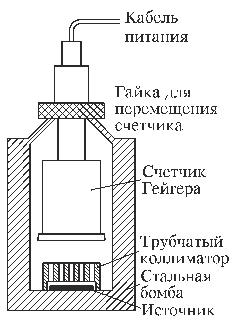
\includegraphics[width=\linewidth]{ustanovka1.pdf}
		\caption{Схема торцевого счетчика Гейгера}
		\label{ris geyger}
	\end{wrapfigure}
	
	Для определения пробега $\alpha$-частиц с помощью счетчика радиоактивный источник помещается на дно стального цилиндра
	(рис. \ref{ris geyger}), в котором может перемещаться счетчик Гейгера.
	
	Импульсы, возникающие в счетчике, усиливаются и регистрируются пересчетной схемой. 
	Изменяя расстояние от счётчика до источника и измеряя зависимость потока частиц от него, мы можем найти энергию частиц и 
	убедиться в скорости их замедления.
	
	\subsection{Ионизационная камера}
	
	Ионизационная камера --- прибор для количественного измерения
	ионизации, произведенной заряженными частицами при прохождении через газ.
	
	Заполняющий сосуд газ сам по себе не проводит электрический ток, 
	ток возникает только при прохождении быстрой заряженной частицы, которая рождает в газе на своем пути ионы.
	
	Поместим на торец внутреннего электрода источник
	ионизирующего излучения, заполним объем камеры воздухом и начнем
	увеличивать разность потенциалов между электродами. 
	Ток, протекающий через камеру, вначале будет резко возрастать, а затем, начиная с некоторого напряжения $ V_0 $, 
	станет постоянным.  Предельный ток $ I_0 $ будет равен $ I_0 = n_0e $,
	где $ n_0 $ --- число пар ионов, образуемых в секунду в объеме камеры, а $ e $ --- заряд электрона.
	
	\begin{wrapfigure}[25]{l}{0.37\linewidth}
		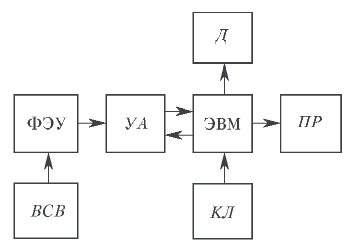
\includegraphics[width=\linewidth]{ustanovka2.pdf}
		\caption{Схема устройства ионизационной камеры}
		\label{ris Ion}
	\end{wrapfigure}
	
	Прохождение тока через камеру регистрируется посредством измерения напряжения на включенном в цепь камеры сопротивлении $ R $.
	Так как средняя энергия ионизации атомов воздуха составляет около 30 эВ, то $\alpha$-частица с энергией 3 МэВ образует на своем пути около $ 10^5 $ электронов, 
	им соответствует заряд $1,6 \cdot 10^{-14} $ Кл. Чтобы столь малое количество заряда, создаваемое проходящей через камеру одной $\alpha$-частицей, 
	вызывало измеряемое напряжение, емкость $ C $ должна быть мала.
	
	\begin{wrapfigure}[15]{r}{0.3\linewidth}
		\includegraphics[width=\linewidth]{PotI}
		\caption{Характерная кривая зависимости
			тока ионизационной камеры от давления.
			Ионизация создается $ \alpha $-частицами}
		\label{ris PotI}
	\end{wrapfigure}
	
	При изменении давления в камере ионизационный ток меняется так, как это показано на рис. \ref{ris PotI}. При небольших давлениях газа
	$\alpha$-частицы передают часть энергии стенкам камеры. По достижении
	давления $ P_0 $ все они заканчивают свой пробег внутри газа, и дальнейшее возрастание тока прекращается. 
	Для определения давления $ P_0 $ чаще всего пользуются методом экстраполяции.
	
	В данной работе измерение пробега $\alpha$-частицы проводится по величине тока ионизации. Внутренним электродом
	камеры служит диск диаметром 5 мм, на который нанесен тонкий слой $ ^{239}_{94} $Pu, покрытый сверху тонкой защитной пленкой. Вторым электродом служит внешняя оболочка камеры. 
	Вакуумная установка содержит кран и манометр. Она позволяет изменять давление в камере.
	Величина тока ионизации измеряется электрометром.
	

	\section{Экспериментальные данные}


	
		\floatsetup[table]{capposition=top}	
		\begin{table}[H]
			\caption{Счетчик Гейгера.}
			\label{table:exp1}
			\begin{tabular}{|r|r|r|r|}
				\hline
				$l$, мм &    $N'$ &    $t$, с & $N$, с$^{-1}$ \\
				\hline
				20 &   14 &   72$\pm0.5$ &   0.195$\pm$0.002 \\ \hline
				 15 &  439 &   30$\pm0.5$ &  14.6$\pm$0.3 \\ \hline
				 11 &  411 &   30$\pm0.5$ &  13.7$\pm$0.3 \\ \hline
				 18 &  242 &   30$\pm0.5$ &   8$\pm$0.2 \\ \hline
				 19 &   42 &   30$\pm0.5$ &   1.4$\pm$0.03\\ \hline
				50 &   12 &  113$\pm0.5$ &   0.106$\pm$0.001 \\ \hline
				 13 &  419 &   30$\pm0.5$ &  14$\pm$0.3 \\ \hline
				 17 &  418 &   30$\pm0.5$ &  14$\pm$0.3 \\ \hline
				25 &   18 &  107$\pm0.5$ &   0.168$\pm$0.001 \\ \hline
				30 &   18 &  107$\pm0.5$ &   0.168$\pm$0.001 \\ \hline
				35 &   22 &   93$\pm0.5$ &   0.237$\pm$0.002 \\ \hline

				\end{tabular}
		\end{table}
	
			\floatsetup[table]{capposition=top}	
		\begin{table}[H]
			\caption{Ионизационная камера.}
			\label{table:exp3}
			\begin{tabular}{|l|r|r|}
				\hline
				$P$, Торр &    $I$, пА \\
				\hline
				 20 &   16 \\ \hline 
				 35 &   42 \\ \hline 
				 60 &   75 \\ \hline 
				 82 &  108 \\ \hline 
				110 &  150 \\ \hline 
				135 &  189 \\ \hline 
				160 &  226 \\ \hline 
				185 &  264 \\ \hline 
				210 &  304 \\ \hline 
				235 &  349 \\ \hline 
				260 &  390 \\ \hline 
				310 &  485 \\ \hline 
				360 &  577 \\ \hline 
				410 &  681 \\ \hline 
				460 &  775 \\ \hline 
				510 &  880 \\ \hline 
				560 &  960 \\ \hline 
				610 &  970 \\ \hline 
				590 &  970 \\ \hline 
				540 &  940 \\ \hline 
				580 &  975 \\ \hline 
				570 &  970 \\ \hline 
				670 &  955 \\ \hline 
				650 &  962 \\ \hline 
				630 &  966 \\ \hline 
				685 &  968 \\ \hline 
				710 &  946 \\ \hline 
				730 &  939 \\ \hline 
				750 &  937 \\ \hline 
				\end{tabular}
		\end{table}
	
	В таблицу 1 занесены значения давлений в ионизационной камере и соответствующий этому давлению ток через нее, во 2 таблице указаны значения количества частиц, прошедших через счетчик Гейгера за соответствующий период времени при различных расстояниях до источника. В последнем столбце 2 таблице подсчитано значение количества пролетающих $\alpha$-частиц за одну секудну.

	\section{Обработка результатов}
		\subsection{Исследование пробега $\alpha$-ч. счетчика Гейгера}	
		Представим результаты измерений (табл.~\ref{table:exp1}) зависимости $N=N(x)$ в виде графика. 
		
		\begin{figure}[h!]
			\centering
			\begin{floatrow}
				%% Creator: Matplotlib, PGF backend
%%
%% To include the figure in your LaTeX document, write
%%   \input{<filename>.pgf}
%%
%% Make sure the required packages are loaded in your preamble
%%   \usepackage{pgf}
%%
%% Figures using additional raster images can only be included by \input if
%% they are in the same directory as the main LaTeX file. For loading figures
%% from other directories you can use the `import` package
%%   \usepackage{import}
%%
%% and then include the figures with
%%   \import{<path to file>}{<filename>.pgf}
%%
%% Matplotlib used the following preamble
%%
\begingroup%
\makeatletter%
\begin{pgfpicture}%
\pgfpathrectangle{\pgfpointorigin}{\pgfqpoint{6.000000in}{4.000000in}}%
\pgfusepath{use as bounding box, clip}%
\begin{pgfscope}%
\pgfsetbuttcap%
\pgfsetmiterjoin%
\pgfsetlinewidth{0.000000pt}%
\definecolor{currentstroke}{rgb}{1.000000,1.000000,1.000000}%
\pgfsetstrokecolor{currentstroke}%
\pgfsetstrokeopacity{0.000000}%
\pgfsetdash{}{0pt}%
\pgfpathmoveto{\pgfqpoint{0.000000in}{0.000000in}}%
\pgfpathlineto{\pgfqpoint{6.000000in}{0.000000in}}%
\pgfpathlineto{\pgfqpoint{6.000000in}{4.000000in}}%
\pgfpathlineto{\pgfqpoint{0.000000in}{4.000000in}}%
\pgfpathclose%
\pgfusepath{}%
\end{pgfscope}%
\begin{pgfscope}%
\pgfsetbuttcap%
\pgfsetmiterjoin%
\definecolor{currentfill}{rgb}{1.000000,1.000000,1.000000}%
\pgfsetfillcolor{currentfill}%
\pgfsetlinewidth{0.000000pt}%
\definecolor{currentstroke}{rgb}{0.000000,0.000000,0.000000}%
\pgfsetstrokecolor{currentstroke}%
\pgfsetstrokeopacity{0.000000}%
\pgfsetdash{}{0pt}%
\pgfpathmoveto{\pgfqpoint{0.750000in}{0.500000in}}%
\pgfpathlineto{\pgfqpoint{5.400000in}{0.500000in}}%
\pgfpathlineto{\pgfqpoint{5.400000in}{3.520000in}}%
\pgfpathlineto{\pgfqpoint{0.750000in}{3.520000in}}%
\pgfpathclose%
\pgfusepath{fill}%
\end{pgfscope}%
\begin{pgfscope}%
\pgfpathrectangle{\pgfqpoint{0.750000in}{0.500000in}}{\pgfqpoint{4.650000in}{3.020000in}}%
\pgfusepath{clip}%
\pgfsetbuttcap%
\pgfsetroundjoin%
\pgfsetlinewidth{0.803000pt}%
\definecolor{currentstroke}{rgb}{0.690196,0.690196,0.690196}%
\pgfsetstrokecolor{currentstroke}%
\pgfsetdash{{2.960000pt}{1.280000pt}}{0.000000pt}%
\pgfpathmoveto{\pgfqpoint{0.961364in}{0.500000in}}%
\pgfpathlineto{\pgfqpoint{0.961364in}{3.520000in}}%
\pgfusepath{stroke}%
\end{pgfscope}%
\begin{pgfscope}%
\pgfsetbuttcap%
\pgfsetroundjoin%
\definecolor{currentfill}{rgb}{0.000000,0.000000,0.000000}%
\pgfsetfillcolor{currentfill}%
\pgfsetlinewidth{0.803000pt}%
\definecolor{currentstroke}{rgb}{0.000000,0.000000,0.000000}%
\pgfsetstrokecolor{currentstroke}%
\pgfsetdash{}{0pt}%
\pgfsys@defobject{currentmarker}{\pgfqpoint{0.000000in}{-0.048611in}}{\pgfqpoint{0.000000in}{0.000000in}}{%
\pgfpathmoveto{\pgfqpoint{0.000000in}{0.000000in}}%
\pgfpathlineto{\pgfqpoint{0.000000in}{-0.048611in}}%
\pgfusepath{stroke,fill}%
}%
\begin{pgfscope}%
\pgfsys@transformshift{0.961364in}{0.500000in}%
\pgfsys@useobject{currentmarker}{}%
\end{pgfscope}%
\end{pgfscope}%
\begin{pgfscope}%
\definecolor{textcolor}{rgb}{0.000000,0.000000,0.000000}%
\pgfsetstrokecolor{textcolor}%
\pgfsetfillcolor{textcolor}%
\pgftext[x=0.961364in,y=0.402778in,,top]{\color{textcolor}\rmfamily\fontsize{10.000000}{12.000000}\selectfont \(\displaystyle {0}\)}%
\end{pgfscope}%
\begin{pgfscope}%
\pgfpathrectangle{\pgfqpoint{0.750000in}{0.500000in}}{\pgfqpoint{4.650000in}{3.020000in}}%
\pgfusepath{clip}%
\pgfsetbuttcap%
\pgfsetroundjoin%
\pgfsetlinewidth{0.803000pt}%
\definecolor{currentstroke}{rgb}{0.690196,0.690196,0.690196}%
\pgfsetstrokecolor{currentstroke}%
\pgfsetdash{{2.960000pt}{1.280000pt}}{0.000000pt}%
\pgfpathmoveto{\pgfqpoint{1.806818in}{0.500000in}}%
\pgfpathlineto{\pgfqpoint{1.806818in}{3.520000in}}%
\pgfusepath{stroke}%
\end{pgfscope}%
\begin{pgfscope}%
\pgfsetbuttcap%
\pgfsetroundjoin%
\definecolor{currentfill}{rgb}{0.000000,0.000000,0.000000}%
\pgfsetfillcolor{currentfill}%
\pgfsetlinewidth{0.803000pt}%
\definecolor{currentstroke}{rgb}{0.000000,0.000000,0.000000}%
\pgfsetstrokecolor{currentstroke}%
\pgfsetdash{}{0pt}%
\pgfsys@defobject{currentmarker}{\pgfqpoint{0.000000in}{-0.048611in}}{\pgfqpoint{0.000000in}{0.000000in}}{%
\pgfpathmoveto{\pgfqpoint{0.000000in}{0.000000in}}%
\pgfpathlineto{\pgfqpoint{0.000000in}{-0.048611in}}%
\pgfusepath{stroke,fill}%
}%
\begin{pgfscope}%
\pgfsys@transformshift{1.806818in}{0.500000in}%
\pgfsys@useobject{currentmarker}{}%
\end{pgfscope}%
\end{pgfscope}%
\begin{pgfscope}%
\definecolor{textcolor}{rgb}{0.000000,0.000000,0.000000}%
\pgfsetstrokecolor{textcolor}%
\pgfsetfillcolor{textcolor}%
\pgftext[x=1.806818in,y=0.402778in,,top]{\color{textcolor}\rmfamily\fontsize{10.000000}{12.000000}\selectfont \(\displaystyle {10}\)}%
\end{pgfscope}%
\begin{pgfscope}%
\pgfpathrectangle{\pgfqpoint{0.750000in}{0.500000in}}{\pgfqpoint{4.650000in}{3.020000in}}%
\pgfusepath{clip}%
\pgfsetbuttcap%
\pgfsetroundjoin%
\pgfsetlinewidth{0.803000pt}%
\definecolor{currentstroke}{rgb}{0.690196,0.690196,0.690196}%
\pgfsetstrokecolor{currentstroke}%
\pgfsetdash{{2.960000pt}{1.280000pt}}{0.000000pt}%
\pgfpathmoveto{\pgfqpoint{2.652273in}{0.500000in}}%
\pgfpathlineto{\pgfqpoint{2.652273in}{3.520000in}}%
\pgfusepath{stroke}%
\end{pgfscope}%
\begin{pgfscope}%
\pgfsetbuttcap%
\pgfsetroundjoin%
\definecolor{currentfill}{rgb}{0.000000,0.000000,0.000000}%
\pgfsetfillcolor{currentfill}%
\pgfsetlinewidth{0.803000pt}%
\definecolor{currentstroke}{rgb}{0.000000,0.000000,0.000000}%
\pgfsetstrokecolor{currentstroke}%
\pgfsetdash{}{0pt}%
\pgfsys@defobject{currentmarker}{\pgfqpoint{0.000000in}{-0.048611in}}{\pgfqpoint{0.000000in}{0.000000in}}{%
\pgfpathmoveto{\pgfqpoint{0.000000in}{0.000000in}}%
\pgfpathlineto{\pgfqpoint{0.000000in}{-0.048611in}}%
\pgfusepath{stroke,fill}%
}%
\begin{pgfscope}%
\pgfsys@transformshift{2.652273in}{0.500000in}%
\pgfsys@useobject{currentmarker}{}%
\end{pgfscope}%
\end{pgfscope}%
\begin{pgfscope}%
\definecolor{textcolor}{rgb}{0.000000,0.000000,0.000000}%
\pgfsetstrokecolor{textcolor}%
\pgfsetfillcolor{textcolor}%
\pgftext[x=2.652273in,y=0.402778in,,top]{\color{textcolor}\rmfamily\fontsize{10.000000}{12.000000}\selectfont \(\displaystyle {20}\)}%
\end{pgfscope}%
\begin{pgfscope}%
\pgfpathrectangle{\pgfqpoint{0.750000in}{0.500000in}}{\pgfqpoint{4.650000in}{3.020000in}}%
\pgfusepath{clip}%
\pgfsetbuttcap%
\pgfsetroundjoin%
\pgfsetlinewidth{0.803000pt}%
\definecolor{currentstroke}{rgb}{0.690196,0.690196,0.690196}%
\pgfsetstrokecolor{currentstroke}%
\pgfsetdash{{2.960000pt}{1.280000pt}}{0.000000pt}%
\pgfpathmoveto{\pgfqpoint{3.497727in}{0.500000in}}%
\pgfpathlineto{\pgfqpoint{3.497727in}{3.520000in}}%
\pgfusepath{stroke}%
\end{pgfscope}%
\begin{pgfscope}%
\pgfsetbuttcap%
\pgfsetroundjoin%
\definecolor{currentfill}{rgb}{0.000000,0.000000,0.000000}%
\pgfsetfillcolor{currentfill}%
\pgfsetlinewidth{0.803000pt}%
\definecolor{currentstroke}{rgb}{0.000000,0.000000,0.000000}%
\pgfsetstrokecolor{currentstroke}%
\pgfsetdash{}{0pt}%
\pgfsys@defobject{currentmarker}{\pgfqpoint{0.000000in}{-0.048611in}}{\pgfqpoint{0.000000in}{0.000000in}}{%
\pgfpathmoveto{\pgfqpoint{0.000000in}{0.000000in}}%
\pgfpathlineto{\pgfqpoint{0.000000in}{-0.048611in}}%
\pgfusepath{stroke,fill}%
}%
\begin{pgfscope}%
\pgfsys@transformshift{3.497727in}{0.500000in}%
\pgfsys@useobject{currentmarker}{}%
\end{pgfscope}%
\end{pgfscope}%
\begin{pgfscope}%
\definecolor{textcolor}{rgb}{0.000000,0.000000,0.000000}%
\pgfsetstrokecolor{textcolor}%
\pgfsetfillcolor{textcolor}%
\pgftext[x=3.497727in,y=0.402778in,,top]{\color{textcolor}\rmfamily\fontsize{10.000000}{12.000000}\selectfont \(\displaystyle {30}\)}%
\end{pgfscope}%
\begin{pgfscope}%
\pgfpathrectangle{\pgfqpoint{0.750000in}{0.500000in}}{\pgfqpoint{4.650000in}{3.020000in}}%
\pgfusepath{clip}%
\pgfsetbuttcap%
\pgfsetroundjoin%
\pgfsetlinewidth{0.803000pt}%
\definecolor{currentstroke}{rgb}{0.690196,0.690196,0.690196}%
\pgfsetstrokecolor{currentstroke}%
\pgfsetdash{{2.960000pt}{1.280000pt}}{0.000000pt}%
\pgfpathmoveto{\pgfqpoint{4.343182in}{0.500000in}}%
\pgfpathlineto{\pgfqpoint{4.343182in}{3.520000in}}%
\pgfusepath{stroke}%
\end{pgfscope}%
\begin{pgfscope}%
\pgfsetbuttcap%
\pgfsetroundjoin%
\definecolor{currentfill}{rgb}{0.000000,0.000000,0.000000}%
\pgfsetfillcolor{currentfill}%
\pgfsetlinewidth{0.803000pt}%
\definecolor{currentstroke}{rgb}{0.000000,0.000000,0.000000}%
\pgfsetstrokecolor{currentstroke}%
\pgfsetdash{}{0pt}%
\pgfsys@defobject{currentmarker}{\pgfqpoint{0.000000in}{-0.048611in}}{\pgfqpoint{0.000000in}{0.000000in}}{%
\pgfpathmoveto{\pgfqpoint{0.000000in}{0.000000in}}%
\pgfpathlineto{\pgfqpoint{0.000000in}{-0.048611in}}%
\pgfusepath{stroke,fill}%
}%
\begin{pgfscope}%
\pgfsys@transformshift{4.343182in}{0.500000in}%
\pgfsys@useobject{currentmarker}{}%
\end{pgfscope}%
\end{pgfscope}%
\begin{pgfscope}%
\definecolor{textcolor}{rgb}{0.000000,0.000000,0.000000}%
\pgfsetstrokecolor{textcolor}%
\pgfsetfillcolor{textcolor}%
\pgftext[x=4.343182in,y=0.402778in,,top]{\color{textcolor}\rmfamily\fontsize{10.000000}{12.000000}\selectfont \(\displaystyle {40}\)}%
\end{pgfscope}%
\begin{pgfscope}%
\pgfpathrectangle{\pgfqpoint{0.750000in}{0.500000in}}{\pgfqpoint{4.650000in}{3.020000in}}%
\pgfusepath{clip}%
\pgfsetbuttcap%
\pgfsetroundjoin%
\pgfsetlinewidth{0.803000pt}%
\definecolor{currentstroke}{rgb}{0.690196,0.690196,0.690196}%
\pgfsetstrokecolor{currentstroke}%
\pgfsetdash{{2.960000pt}{1.280000pt}}{0.000000pt}%
\pgfpathmoveto{\pgfqpoint{5.188636in}{0.500000in}}%
\pgfpathlineto{\pgfqpoint{5.188636in}{3.520000in}}%
\pgfusepath{stroke}%
\end{pgfscope}%
\begin{pgfscope}%
\pgfsetbuttcap%
\pgfsetroundjoin%
\definecolor{currentfill}{rgb}{0.000000,0.000000,0.000000}%
\pgfsetfillcolor{currentfill}%
\pgfsetlinewidth{0.803000pt}%
\definecolor{currentstroke}{rgb}{0.000000,0.000000,0.000000}%
\pgfsetstrokecolor{currentstroke}%
\pgfsetdash{}{0pt}%
\pgfsys@defobject{currentmarker}{\pgfqpoint{0.000000in}{-0.048611in}}{\pgfqpoint{0.000000in}{0.000000in}}{%
\pgfpathmoveto{\pgfqpoint{0.000000in}{0.000000in}}%
\pgfpathlineto{\pgfqpoint{0.000000in}{-0.048611in}}%
\pgfusepath{stroke,fill}%
}%
\begin{pgfscope}%
\pgfsys@transformshift{5.188636in}{0.500000in}%
\pgfsys@useobject{currentmarker}{}%
\end{pgfscope}%
\end{pgfscope}%
\begin{pgfscope}%
\definecolor{textcolor}{rgb}{0.000000,0.000000,0.000000}%
\pgfsetstrokecolor{textcolor}%
\pgfsetfillcolor{textcolor}%
\pgftext[x=5.188636in,y=0.402778in,,top]{\color{textcolor}\rmfamily\fontsize{10.000000}{12.000000}\selectfont \(\displaystyle {50}\)}%
\end{pgfscope}%
\begin{pgfscope}%
\definecolor{textcolor}{rgb}{0.000000,0.000000,0.000000}%
\pgfsetstrokecolor{textcolor}%
\pgfsetfillcolor{textcolor}%
\pgftext[x=3.075000in,y=0.223766in,,top]{\color{textcolor}\rmfamily\fontsize{10.000000}{12.000000}\selectfont \(\displaystyle l, cm\)}%
\end{pgfscope}%
\begin{pgfscope}%
\pgfpathrectangle{\pgfqpoint{0.750000in}{0.500000in}}{\pgfqpoint{4.650000in}{3.020000in}}%
\pgfusepath{clip}%
\pgfsetbuttcap%
\pgfsetroundjoin%
\pgfsetlinewidth{0.803000pt}%
\definecolor{currentstroke}{rgb}{0.690196,0.690196,0.690196}%
\pgfsetstrokecolor{currentstroke}%
\pgfsetdash{{2.960000pt}{1.280000pt}}{0.000000pt}%
\pgfpathmoveto{\pgfqpoint{0.750000in}{0.637273in}}%
\pgfpathlineto{\pgfqpoint{5.400000in}{0.637273in}}%
\pgfusepath{stroke}%
\end{pgfscope}%
\begin{pgfscope}%
\pgfsetbuttcap%
\pgfsetroundjoin%
\definecolor{currentfill}{rgb}{0.000000,0.000000,0.000000}%
\pgfsetfillcolor{currentfill}%
\pgfsetlinewidth{0.803000pt}%
\definecolor{currentstroke}{rgb}{0.000000,0.000000,0.000000}%
\pgfsetstrokecolor{currentstroke}%
\pgfsetdash{}{0pt}%
\pgfsys@defobject{currentmarker}{\pgfqpoint{-0.048611in}{0.000000in}}{\pgfqpoint{-0.000000in}{0.000000in}}{%
\pgfpathmoveto{\pgfqpoint{-0.000000in}{0.000000in}}%
\pgfpathlineto{\pgfqpoint{-0.048611in}{0.000000in}}%
\pgfusepath{stroke,fill}%
}%
\begin{pgfscope}%
\pgfsys@transformshift{0.750000in}{0.637273in}%
\pgfsys@useobject{currentmarker}{}%
\end{pgfscope}%
\end{pgfscope}%
\begin{pgfscope}%
\definecolor{textcolor}{rgb}{0.000000,0.000000,0.000000}%
\pgfsetstrokecolor{textcolor}%
\pgfsetfillcolor{textcolor}%
\pgftext[x=0.583333in, y=0.589047in, left, base]{\color{textcolor}\rmfamily\fontsize{10.000000}{12.000000}\selectfont \(\displaystyle {0}\)}%
\end{pgfscope}%
\begin{pgfscope}%
\pgfpathrectangle{\pgfqpoint{0.750000in}{0.500000in}}{\pgfqpoint{4.650000in}{3.020000in}}%
\pgfusepath{clip}%
\pgfsetbuttcap%
\pgfsetroundjoin%
\pgfsetlinewidth{0.803000pt}%
\definecolor{currentstroke}{rgb}{0.690196,0.690196,0.690196}%
\pgfsetstrokecolor{currentstroke}%
\pgfsetdash{{2.960000pt}{1.280000pt}}{0.000000pt}%
\pgfpathmoveto{\pgfqpoint{0.750000in}{1.000401in}}%
\pgfpathlineto{\pgfqpoint{5.400000in}{1.000401in}}%
\pgfusepath{stroke}%
\end{pgfscope}%
\begin{pgfscope}%
\pgfsetbuttcap%
\pgfsetroundjoin%
\definecolor{currentfill}{rgb}{0.000000,0.000000,0.000000}%
\pgfsetfillcolor{currentfill}%
\pgfsetlinewidth{0.803000pt}%
\definecolor{currentstroke}{rgb}{0.000000,0.000000,0.000000}%
\pgfsetstrokecolor{currentstroke}%
\pgfsetdash{}{0pt}%
\pgfsys@defobject{currentmarker}{\pgfqpoint{-0.048611in}{0.000000in}}{\pgfqpoint{-0.000000in}{0.000000in}}{%
\pgfpathmoveto{\pgfqpoint{-0.000000in}{0.000000in}}%
\pgfpathlineto{\pgfqpoint{-0.048611in}{0.000000in}}%
\pgfusepath{stroke,fill}%
}%
\begin{pgfscope}%
\pgfsys@transformshift{0.750000in}{1.000401in}%
\pgfsys@useobject{currentmarker}{}%
\end{pgfscope}%
\end{pgfscope}%
\begin{pgfscope}%
\definecolor{textcolor}{rgb}{0.000000,0.000000,0.000000}%
\pgfsetstrokecolor{textcolor}%
\pgfsetfillcolor{textcolor}%
\pgftext[x=0.583333in, y=0.952176in, left, base]{\color{textcolor}\rmfamily\fontsize{10.000000}{12.000000}\selectfont \(\displaystyle {2}\)}%
\end{pgfscope}%
\begin{pgfscope}%
\pgfpathrectangle{\pgfqpoint{0.750000in}{0.500000in}}{\pgfqpoint{4.650000in}{3.020000in}}%
\pgfusepath{clip}%
\pgfsetbuttcap%
\pgfsetroundjoin%
\pgfsetlinewidth{0.803000pt}%
\definecolor{currentstroke}{rgb}{0.690196,0.690196,0.690196}%
\pgfsetstrokecolor{currentstroke}%
\pgfsetdash{{2.960000pt}{1.280000pt}}{0.000000pt}%
\pgfpathmoveto{\pgfqpoint{0.750000in}{1.363530in}}%
\pgfpathlineto{\pgfqpoint{5.400000in}{1.363530in}}%
\pgfusepath{stroke}%
\end{pgfscope}%
\begin{pgfscope}%
\pgfsetbuttcap%
\pgfsetroundjoin%
\definecolor{currentfill}{rgb}{0.000000,0.000000,0.000000}%
\pgfsetfillcolor{currentfill}%
\pgfsetlinewidth{0.803000pt}%
\definecolor{currentstroke}{rgb}{0.000000,0.000000,0.000000}%
\pgfsetstrokecolor{currentstroke}%
\pgfsetdash{}{0pt}%
\pgfsys@defobject{currentmarker}{\pgfqpoint{-0.048611in}{0.000000in}}{\pgfqpoint{-0.000000in}{0.000000in}}{%
\pgfpathmoveto{\pgfqpoint{-0.000000in}{0.000000in}}%
\pgfpathlineto{\pgfqpoint{-0.048611in}{0.000000in}}%
\pgfusepath{stroke,fill}%
}%
\begin{pgfscope}%
\pgfsys@transformshift{0.750000in}{1.363530in}%
\pgfsys@useobject{currentmarker}{}%
\end{pgfscope}%
\end{pgfscope}%
\begin{pgfscope}%
\definecolor{textcolor}{rgb}{0.000000,0.000000,0.000000}%
\pgfsetstrokecolor{textcolor}%
\pgfsetfillcolor{textcolor}%
\pgftext[x=0.583333in, y=1.315305in, left, base]{\color{textcolor}\rmfamily\fontsize{10.000000}{12.000000}\selectfont \(\displaystyle {4}\)}%
\end{pgfscope}%
\begin{pgfscope}%
\pgfpathrectangle{\pgfqpoint{0.750000in}{0.500000in}}{\pgfqpoint{4.650000in}{3.020000in}}%
\pgfusepath{clip}%
\pgfsetbuttcap%
\pgfsetroundjoin%
\pgfsetlinewidth{0.803000pt}%
\definecolor{currentstroke}{rgb}{0.690196,0.690196,0.690196}%
\pgfsetstrokecolor{currentstroke}%
\pgfsetdash{{2.960000pt}{1.280000pt}}{0.000000pt}%
\pgfpathmoveto{\pgfqpoint{0.750000in}{1.726659in}}%
\pgfpathlineto{\pgfqpoint{5.400000in}{1.726659in}}%
\pgfusepath{stroke}%
\end{pgfscope}%
\begin{pgfscope}%
\pgfsetbuttcap%
\pgfsetroundjoin%
\definecolor{currentfill}{rgb}{0.000000,0.000000,0.000000}%
\pgfsetfillcolor{currentfill}%
\pgfsetlinewidth{0.803000pt}%
\definecolor{currentstroke}{rgb}{0.000000,0.000000,0.000000}%
\pgfsetstrokecolor{currentstroke}%
\pgfsetdash{}{0pt}%
\pgfsys@defobject{currentmarker}{\pgfqpoint{-0.048611in}{0.000000in}}{\pgfqpoint{-0.000000in}{0.000000in}}{%
\pgfpathmoveto{\pgfqpoint{-0.000000in}{0.000000in}}%
\pgfpathlineto{\pgfqpoint{-0.048611in}{0.000000in}}%
\pgfusepath{stroke,fill}%
}%
\begin{pgfscope}%
\pgfsys@transformshift{0.750000in}{1.726659in}%
\pgfsys@useobject{currentmarker}{}%
\end{pgfscope}%
\end{pgfscope}%
\begin{pgfscope}%
\definecolor{textcolor}{rgb}{0.000000,0.000000,0.000000}%
\pgfsetstrokecolor{textcolor}%
\pgfsetfillcolor{textcolor}%
\pgftext[x=0.583333in, y=1.678433in, left, base]{\color{textcolor}\rmfamily\fontsize{10.000000}{12.000000}\selectfont \(\displaystyle {6}\)}%
\end{pgfscope}%
\begin{pgfscope}%
\pgfpathrectangle{\pgfqpoint{0.750000in}{0.500000in}}{\pgfqpoint{4.650000in}{3.020000in}}%
\pgfusepath{clip}%
\pgfsetbuttcap%
\pgfsetroundjoin%
\pgfsetlinewidth{0.803000pt}%
\definecolor{currentstroke}{rgb}{0.690196,0.690196,0.690196}%
\pgfsetstrokecolor{currentstroke}%
\pgfsetdash{{2.960000pt}{1.280000pt}}{0.000000pt}%
\pgfpathmoveto{\pgfqpoint{0.750000in}{2.089787in}}%
\pgfpathlineto{\pgfqpoint{5.400000in}{2.089787in}}%
\pgfusepath{stroke}%
\end{pgfscope}%
\begin{pgfscope}%
\pgfsetbuttcap%
\pgfsetroundjoin%
\definecolor{currentfill}{rgb}{0.000000,0.000000,0.000000}%
\pgfsetfillcolor{currentfill}%
\pgfsetlinewidth{0.803000pt}%
\definecolor{currentstroke}{rgb}{0.000000,0.000000,0.000000}%
\pgfsetstrokecolor{currentstroke}%
\pgfsetdash{}{0pt}%
\pgfsys@defobject{currentmarker}{\pgfqpoint{-0.048611in}{0.000000in}}{\pgfqpoint{-0.000000in}{0.000000in}}{%
\pgfpathmoveto{\pgfqpoint{-0.000000in}{0.000000in}}%
\pgfpathlineto{\pgfqpoint{-0.048611in}{0.000000in}}%
\pgfusepath{stroke,fill}%
}%
\begin{pgfscope}%
\pgfsys@transformshift{0.750000in}{2.089787in}%
\pgfsys@useobject{currentmarker}{}%
\end{pgfscope}%
\end{pgfscope}%
\begin{pgfscope}%
\definecolor{textcolor}{rgb}{0.000000,0.000000,0.000000}%
\pgfsetstrokecolor{textcolor}%
\pgfsetfillcolor{textcolor}%
\pgftext[x=0.583333in, y=2.041562in, left, base]{\color{textcolor}\rmfamily\fontsize{10.000000}{12.000000}\selectfont \(\displaystyle {8}\)}%
\end{pgfscope}%
\begin{pgfscope}%
\pgfpathrectangle{\pgfqpoint{0.750000in}{0.500000in}}{\pgfqpoint{4.650000in}{3.020000in}}%
\pgfusepath{clip}%
\pgfsetbuttcap%
\pgfsetroundjoin%
\pgfsetlinewidth{0.803000pt}%
\definecolor{currentstroke}{rgb}{0.690196,0.690196,0.690196}%
\pgfsetstrokecolor{currentstroke}%
\pgfsetdash{{2.960000pt}{1.280000pt}}{0.000000pt}%
\pgfpathmoveto{\pgfqpoint{0.750000in}{2.452916in}}%
\pgfpathlineto{\pgfqpoint{5.400000in}{2.452916in}}%
\pgfusepath{stroke}%
\end{pgfscope}%
\begin{pgfscope}%
\pgfsetbuttcap%
\pgfsetroundjoin%
\definecolor{currentfill}{rgb}{0.000000,0.000000,0.000000}%
\pgfsetfillcolor{currentfill}%
\pgfsetlinewidth{0.803000pt}%
\definecolor{currentstroke}{rgb}{0.000000,0.000000,0.000000}%
\pgfsetstrokecolor{currentstroke}%
\pgfsetdash{}{0pt}%
\pgfsys@defobject{currentmarker}{\pgfqpoint{-0.048611in}{0.000000in}}{\pgfqpoint{-0.000000in}{0.000000in}}{%
\pgfpathmoveto{\pgfqpoint{-0.000000in}{0.000000in}}%
\pgfpathlineto{\pgfqpoint{-0.048611in}{0.000000in}}%
\pgfusepath{stroke,fill}%
}%
\begin{pgfscope}%
\pgfsys@transformshift{0.750000in}{2.452916in}%
\pgfsys@useobject{currentmarker}{}%
\end{pgfscope}%
\end{pgfscope}%
\begin{pgfscope}%
\definecolor{textcolor}{rgb}{0.000000,0.000000,0.000000}%
\pgfsetstrokecolor{textcolor}%
\pgfsetfillcolor{textcolor}%
\pgftext[x=0.513888in, y=2.404691in, left, base]{\color{textcolor}\rmfamily\fontsize{10.000000}{12.000000}\selectfont \(\displaystyle {10}\)}%
\end{pgfscope}%
\begin{pgfscope}%
\pgfpathrectangle{\pgfqpoint{0.750000in}{0.500000in}}{\pgfqpoint{4.650000in}{3.020000in}}%
\pgfusepath{clip}%
\pgfsetbuttcap%
\pgfsetroundjoin%
\pgfsetlinewidth{0.803000pt}%
\definecolor{currentstroke}{rgb}{0.690196,0.690196,0.690196}%
\pgfsetstrokecolor{currentstroke}%
\pgfsetdash{{2.960000pt}{1.280000pt}}{0.000000pt}%
\pgfpathmoveto{\pgfqpoint{0.750000in}{2.816045in}}%
\pgfpathlineto{\pgfqpoint{5.400000in}{2.816045in}}%
\pgfusepath{stroke}%
\end{pgfscope}%
\begin{pgfscope}%
\pgfsetbuttcap%
\pgfsetroundjoin%
\definecolor{currentfill}{rgb}{0.000000,0.000000,0.000000}%
\pgfsetfillcolor{currentfill}%
\pgfsetlinewidth{0.803000pt}%
\definecolor{currentstroke}{rgb}{0.000000,0.000000,0.000000}%
\pgfsetstrokecolor{currentstroke}%
\pgfsetdash{}{0pt}%
\pgfsys@defobject{currentmarker}{\pgfqpoint{-0.048611in}{0.000000in}}{\pgfqpoint{-0.000000in}{0.000000in}}{%
\pgfpathmoveto{\pgfqpoint{-0.000000in}{0.000000in}}%
\pgfpathlineto{\pgfqpoint{-0.048611in}{0.000000in}}%
\pgfusepath{stroke,fill}%
}%
\begin{pgfscope}%
\pgfsys@transformshift{0.750000in}{2.816045in}%
\pgfsys@useobject{currentmarker}{}%
\end{pgfscope}%
\end{pgfscope}%
\begin{pgfscope}%
\definecolor{textcolor}{rgb}{0.000000,0.000000,0.000000}%
\pgfsetstrokecolor{textcolor}%
\pgfsetfillcolor{textcolor}%
\pgftext[x=0.513888in, y=2.767820in, left, base]{\color{textcolor}\rmfamily\fontsize{10.000000}{12.000000}\selectfont \(\displaystyle {12}\)}%
\end{pgfscope}%
\begin{pgfscope}%
\pgfpathrectangle{\pgfqpoint{0.750000in}{0.500000in}}{\pgfqpoint{4.650000in}{3.020000in}}%
\pgfusepath{clip}%
\pgfsetbuttcap%
\pgfsetroundjoin%
\pgfsetlinewidth{0.803000pt}%
\definecolor{currentstroke}{rgb}{0.690196,0.690196,0.690196}%
\pgfsetstrokecolor{currentstroke}%
\pgfsetdash{{2.960000pt}{1.280000pt}}{0.000000pt}%
\pgfpathmoveto{\pgfqpoint{0.750000in}{3.179173in}}%
\pgfpathlineto{\pgfqpoint{5.400000in}{3.179173in}}%
\pgfusepath{stroke}%
\end{pgfscope}%
\begin{pgfscope}%
\pgfsetbuttcap%
\pgfsetroundjoin%
\definecolor{currentfill}{rgb}{0.000000,0.000000,0.000000}%
\pgfsetfillcolor{currentfill}%
\pgfsetlinewidth{0.803000pt}%
\definecolor{currentstroke}{rgb}{0.000000,0.000000,0.000000}%
\pgfsetstrokecolor{currentstroke}%
\pgfsetdash{}{0pt}%
\pgfsys@defobject{currentmarker}{\pgfqpoint{-0.048611in}{0.000000in}}{\pgfqpoint{-0.000000in}{0.000000in}}{%
\pgfpathmoveto{\pgfqpoint{-0.000000in}{0.000000in}}%
\pgfpathlineto{\pgfqpoint{-0.048611in}{0.000000in}}%
\pgfusepath{stroke,fill}%
}%
\begin{pgfscope}%
\pgfsys@transformshift{0.750000in}{3.179173in}%
\pgfsys@useobject{currentmarker}{}%
\end{pgfscope}%
\end{pgfscope}%
\begin{pgfscope}%
\definecolor{textcolor}{rgb}{0.000000,0.000000,0.000000}%
\pgfsetstrokecolor{textcolor}%
\pgfsetfillcolor{textcolor}%
\pgftext[x=0.513888in, y=3.130948in, left, base]{\color{textcolor}\rmfamily\fontsize{10.000000}{12.000000}\selectfont \(\displaystyle {14}\)}%
\end{pgfscope}%
\begin{pgfscope}%
\definecolor{textcolor}{rgb}{0.000000,0.000000,0.000000}%
\pgfsetstrokecolor{textcolor}%
\pgfsetfillcolor{textcolor}%
\pgftext[x=0.458333in,y=2.010000in,,bottom,rotate=90.000000]{\color{textcolor}\rmfamily\fontsize{10.000000}{12.000000}\selectfont \(\displaystyle N\)}%
\end{pgfscope}%
\begin{pgfscope}%
\pgfpathrectangle{\pgfqpoint{0.750000in}{0.500000in}}{\pgfqpoint{4.650000in}{3.020000in}}%
\pgfusepath{clip}%
\pgfsetbuttcap%
\pgfsetroundjoin%
\pgfsetlinewidth{1.003750pt}%
\definecolor{currentstroke}{rgb}{0.000000,0.000000,0.000000}%
\pgfsetstrokecolor{currentstroke}%
\pgfsetdash{}{0pt}%
\pgfpathmoveto{\pgfqpoint{1.806818in}{0.672087in}}%
\pgfpathlineto{\pgfqpoint{1.806818in}{0.673067in}}%
\pgfusepath{stroke}%
\end{pgfscope}%
\begin{pgfscope}%
\pgfpathrectangle{\pgfqpoint{0.750000in}{0.500000in}}{\pgfqpoint{4.650000in}{3.020000in}}%
\pgfusepath{clip}%
\pgfsetbuttcap%
\pgfsetroundjoin%
\pgfsetlinewidth{1.003750pt}%
\definecolor{currentstroke}{rgb}{0.000000,0.000000,0.000000}%
\pgfsetstrokecolor{currentstroke}%
\pgfsetdash{}{0pt}%
\pgfpathmoveto{\pgfqpoint{1.384091in}{3.205601in}}%
\pgfpathlineto{\pgfqpoint{1.384091in}{3.382727in}}%
\pgfusepath{stroke}%
\end{pgfscope}%
\begin{pgfscope}%
\pgfpathrectangle{\pgfqpoint{0.750000in}{0.500000in}}{\pgfqpoint{4.650000in}{3.020000in}}%
\pgfusepath{clip}%
\pgfsetbuttcap%
\pgfsetroundjoin%
\pgfsetlinewidth{1.003750pt}%
\definecolor{currentstroke}{rgb}{0.000000,0.000000,0.000000}%
\pgfsetstrokecolor{currentstroke}%
\pgfsetdash{}{0pt}%
\pgfpathmoveto{\pgfqpoint{1.045909in}{3.041790in}}%
\pgfpathlineto{\pgfqpoint{1.045909in}{3.207619in}}%
\pgfusepath{stroke}%
\end{pgfscope}%
\begin{pgfscope}%
\pgfpathrectangle{\pgfqpoint{0.750000in}{0.500000in}}{\pgfqpoint{4.650000in}{3.020000in}}%
\pgfusepath{clip}%
\pgfsetbuttcap%
\pgfsetroundjoin%
\pgfsetlinewidth{1.003750pt}%
\definecolor{currentstroke}{rgb}{0.000000,0.000000,0.000000}%
\pgfsetstrokecolor{currentstroke}%
\pgfsetdash{}{0pt}%
\pgfpathmoveto{\pgfqpoint{1.637727in}{2.053071in}}%
\pgfpathlineto{\pgfqpoint{1.637727in}{2.150712in}}%
\pgfusepath{stroke}%
\end{pgfscope}%
\begin{pgfscope}%
\pgfpathrectangle{\pgfqpoint{0.750000in}{0.500000in}}{\pgfqpoint{4.650000in}{3.020000in}}%
\pgfusepath{clip}%
\pgfsetbuttcap%
\pgfsetroundjoin%
\pgfsetlinewidth{1.003750pt}%
\definecolor{currentstroke}{rgb}{0.000000,0.000000,0.000000}%
\pgfsetstrokecolor{currentstroke}%
\pgfsetdash{}{0pt}%
\pgfpathmoveto{\pgfqpoint{1.722273in}{0.882990in}}%
\pgfpathlineto{\pgfqpoint{1.722273in}{0.899936in}}%
\pgfusepath{stroke}%
\end{pgfscope}%
\begin{pgfscope}%
\pgfpathrectangle{\pgfqpoint{0.750000in}{0.500000in}}{\pgfqpoint{4.650000in}{3.020000in}}%
\pgfusepath{clip}%
\pgfsetbuttcap%
\pgfsetroundjoin%
\pgfsetlinewidth{1.003750pt}%
\definecolor{currentstroke}{rgb}{0.000000,0.000000,0.000000}%
\pgfsetstrokecolor{currentstroke}%
\pgfsetdash{}{0pt}%
\pgfpathmoveto{\pgfqpoint{4.343182in}{0.656383in}}%
\pgfpathlineto{\pgfqpoint{4.343182in}{0.656725in}}%
\pgfusepath{stroke}%
\end{pgfscope}%
\begin{pgfscope}%
\pgfpathrectangle{\pgfqpoint{0.750000in}{0.500000in}}{\pgfqpoint{4.650000in}{3.020000in}}%
\pgfusepath{clip}%
\pgfsetbuttcap%
\pgfsetroundjoin%
\pgfsetlinewidth{1.003750pt}%
\definecolor{currentstroke}{rgb}{0.000000,0.000000,0.000000}%
\pgfsetstrokecolor{currentstroke}%
\pgfsetdash{}{0pt}%
\pgfpathmoveto{\pgfqpoint{1.215000in}{3.088593in}}%
\pgfpathlineto{\pgfqpoint{1.215000in}{3.257650in}}%
\pgfusepath{stroke}%
\end{pgfscope}%
\begin{pgfscope}%
\pgfpathrectangle{\pgfqpoint{0.750000in}{0.500000in}}{\pgfqpoint{4.650000in}{3.020000in}}%
\pgfusepath{clip}%
\pgfsetbuttcap%
\pgfsetroundjoin%
\pgfsetlinewidth{1.003750pt}%
\definecolor{currentstroke}{rgb}{0.000000,0.000000,0.000000}%
\pgfsetstrokecolor{currentstroke}%
\pgfsetdash{}{0pt}%
\pgfpathmoveto{\pgfqpoint{1.553182in}{3.082743in}}%
\pgfpathlineto{\pgfqpoint{1.553182in}{3.251396in}}%
\pgfusepath{stroke}%
\end{pgfscope}%
\begin{pgfscope}%
\pgfpathrectangle{\pgfqpoint{0.750000in}{0.500000in}}{\pgfqpoint{4.650000in}{3.020000in}}%
\pgfusepath{clip}%
\pgfsetbuttcap%
\pgfsetroundjoin%
\pgfsetlinewidth{1.003750pt}%
\definecolor{currentstroke}{rgb}{0.000000,0.000000,0.000000}%
\pgfsetstrokecolor{currentstroke}%
\pgfsetdash{}{0pt}%
\pgfpathmoveto{\pgfqpoint{2.229545in}{0.667531in}}%
\pgfpathlineto{\pgfqpoint{2.229545in}{0.668102in}}%
\pgfusepath{stroke}%
\end{pgfscope}%
\begin{pgfscope}%
\pgfpathrectangle{\pgfqpoint{0.750000in}{0.500000in}}{\pgfqpoint{4.650000in}{3.020000in}}%
\pgfusepath{clip}%
\pgfsetbuttcap%
\pgfsetroundjoin%
\pgfsetlinewidth{1.003750pt}%
\definecolor{currentstroke}{rgb}{0.000000,0.000000,0.000000}%
\pgfsetstrokecolor{currentstroke}%
\pgfsetdash{}{0pt}%
\pgfpathmoveto{\pgfqpoint{2.652273in}{0.667531in}}%
\pgfpathlineto{\pgfqpoint{2.652273in}{0.668102in}}%
\pgfusepath{stroke}%
\end{pgfscope}%
\begin{pgfscope}%
\pgfpathrectangle{\pgfqpoint{0.750000in}{0.500000in}}{\pgfqpoint{4.650000in}{3.020000in}}%
\pgfusepath{clip}%
\pgfsetbuttcap%
\pgfsetroundjoin%
\pgfsetlinewidth{1.003750pt}%
\definecolor{currentstroke}{rgb}{0.000000,0.000000,0.000000}%
\pgfsetstrokecolor{currentstroke}%
\pgfsetdash{}{0pt}%
\pgfpathmoveto{\pgfqpoint{3.075000in}{0.679762in}}%
\pgfpathlineto{\pgfqpoint{3.075000in}{0.680685in}}%
\pgfusepath{stroke}%
\end{pgfscope}%
\begin{pgfscope}%
\pgfpathrectangle{\pgfqpoint{0.750000in}{0.500000in}}{\pgfqpoint{4.650000in}{3.020000in}}%
\pgfusepath{clip}%
\pgfsetrectcap%
\pgfsetroundjoin%
\pgfsetlinewidth{1.003750pt}%
\definecolor{currentstroke}{rgb}{0.000000,0.000000,0.000000}%
\pgfsetstrokecolor{currentstroke}%
\pgfsetdash{}{0pt}%
\pgfpathmoveto{\pgfqpoint{0.961364in}{3.216195in}}%
\pgfpathlineto{\pgfqpoint{1.004063in}{3.216195in}}%
\pgfpathlineto{\pgfqpoint{1.046763in}{3.216195in}}%
\pgfpathlineto{\pgfqpoint{1.089463in}{3.216195in}}%
\pgfpathlineto{\pgfqpoint{1.132163in}{3.216195in}}%
\pgfpathlineto{\pgfqpoint{1.174862in}{3.216194in}}%
\pgfpathlineto{\pgfqpoint{1.217562in}{3.216192in}}%
\pgfpathlineto{\pgfqpoint{1.260262in}{3.216184in}}%
\pgfpathlineto{\pgfqpoint{1.302961in}{3.216153in}}%
\pgfpathlineto{\pgfqpoint{1.345661in}{3.216032in}}%
\pgfpathlineto{\pgfqpoint{1.388361in}{3.215554in}}%
\pgfpathlineto{\pgfqpoint{1.431061in}{3.213680in}}%
\pgfpathlineto{\pgfqpoint{1.473760in}{3.206353in}}%
\pgfpathlineto{\pgfqpoint{1.516460in}{3.177991in}}%
\pgfpathlineto{\pgfqpoint{1.559160in}{3.072462in}}%
\pgfpathlineto{\pgfqpoint{1.601860in}{2.731098in}}%
\pgfpathlineto{\pgfqpoint{1.644559in}{1.987918in}}%
\pgfpathlineto{\pgfqpoint{1.687259in}{1.201636in}}%
\pgfpathlineto{\pgfqpoint{1.729959in}{0.809068in}}%
\pgfpathlineto{\pgfqpoint{1.772658in}{0.683326in}}%
\pgfpathlineto{\pgfqpoint{1.815358in}{0.649164in}}%
\pgfpathlineto{\pgfqpoint{1.858058in}{0.640312in}}%
\pgfpathlineto{\pgfqpoint{1.900758in}{0.638048in}}%
\pgfpathlineto{\pgfqpoint{1.943457in}{0.637470in}}%
\pgfpathlineto{\pgfqpoint{1.986157in}{0.637323in}}%
\pgfpathlineto{\pgfqpoint{2.028857in}{0.637286in}}%
\pgfpathlineto{\pgfqpoint{2.071556in}{0.637276in}}%
\pgfpathlineto{\pgfqpoint{2.114256in}{0.637274in}}%
\pgfpathlineto{\pgfqpoint{2.156956in}{0.637273in}}%
\pgfpathlineto{\pgfqpoint{2.199656in}{0.637273in}}%
\pgfpathlineto{\pgfqpoint{2.242355in}{0.637273in}}%
\pgfpathlineto{\pgfqpoint{2.285055in}{0.637273in}}%
\pgfpathlineto{\pgfqpoint{2.327755in}{0.637273in}}%
\pgfpathlineto{\pgfqpoint{2.370455in}{0.637273in}}%
\pgfpathlineto{\pgfqpoint{2.413154in}{0.637273in}}%
\pgfpathlineto{\pgfqpoint{2.455854in}{0.637273in}}%
\pgfpathlineto{\pgfqpoint{2.498554in}{0.637273in}}%
\pgfpathlineto{\pgfqpoint{2.541253in}{0.637273in}}%
\pgfpathlineto{\pgfqpoint{2.583953in}{0.637273in}}%
\pgfpathlineto{\pgfqpoint{2.626653in}{0.637273in}}%
\pgfpathlineto{\pgfqpoint{2.669353in}{0.637273in}}%
\pgfpathlineto{\pgfqpoint{2.712052in}{0.637273in}}%
\pgfpathlineto{\pgfqpoint{2.754752in}{0.637273in}}%
\pgfpathlineto{\pgfqpoint{2.797452in}{0.637273in}}%
\pgfpathlineto{\pgfqpoint{2.840152in}{0.637273in}}%
\pgfpathlineto{\pgfqpoint{2.882851in}{0.637273in}}%
\pgfpathlineto{\pgfqpoint{2.925551in}{0.637273in}}%
\pgfpathlineto{\pgfqpoint{2.968251in}{0.637273in}}%
\pgfpathlineto{\pgfqpoint{3.010950in}{0.637273in}}%
\pgfpathlineto{\pgfqpoint{3.053650in}{0.637273in}}%
\pgfpathlineto{\pgfqpoint{3.096350in}{0.637273in}}%
\pgfpathlineto{\pgfqpoint{3.139050in}{0.637273in}}%
\pgfpathlineto{\pgfqpoint{3.181749in}{0.637273in}}%
\pgfpathlineto{\pgfqpoint{3.224449in}{0.637273in}}%
\pgfpathlineto{\pgfqpoint{3.267149in}{0.637273in}}%
\pgfpathlineto{\pgfqpoint{3.309848in}{0.637273in}}%
\pgfpathlineto{\pgfqpoint{3.352548in}{0.637273in}}%
\pgfpathlineto{\pgfqpoint{3.395248in}{0.637273in}}%
\pgfpathlineto{\pgfqpoint{3.437948in}{0.637273in}}%
\pgfpathlineto{\pgfqpoint{3.480647in}{0.637273in}}%
\pgfpathlineto{\pgfqpoint{3.523347in}{0.637273in}}%
\pgfpathlineto{\pgfqpoint{3.566047in}{0.637273in}}%
\pgfpathlineto{\pgfqpoint{3.608747in}{0.637273in}}%
\pgfpathlineto{\pgfqpoint{3.651446in}{0.637273in}}%
\pgfpathlineto{\pgfqpoint{3.694146in}{0.637273in}}%
\pgfpathlineto{\pgfqpoint{3.736846in}{0.637273in}}%
\pgfpathlineto{\pgfqpoint{3.779545in}{0.637273in}}%
\pgfpathlineto{\pgfqpoint{3.822245in}{0.637273in}}%
\pgfpathlineto{\pgfqpoint{3.864945in}{0.637273in}}%
\pgfpathlineto{\pgfqpoint{3.907645in}{0.637273in}}%
\pgfpathlineto{\pgfqpoint{3.950344in}{0.637273in}}%
\pgfpathlineto{\pgfqpoint{3.993044in}{0.637273in}}%
\pgfpathlineto{\pgfqpoint{4.035744in}{0.637273in}}%
\pgfpathlineto{\pgfqpoint{4.078444in}{0.637273in}}%
\pgfpathlineto{\pgfqpoint{4.121143in}{0.637273in}}%
\pgfpathlineto{\pgfqpoint{4.163843in}{0.637273in}}%
\pgfpathlineto{\pgfqpoint{4.206543in}{0.637273in}}%
\pgfpathlineto{\pgfqpoint{4.249242in}{0.637273in}}%
\pgfpathlineto{\pgfqpoint{4.291942in}{0.637273in}}%
\pgfpathlineto{\pgfqpoint{4.334642in}{0.637273in}}%
\pgfpathlineto{\pgfqpoint{4.377342in}{0.637273in}}%
\pgfpathlineto{\pgfqpoint{4.420041in}{0.637273in}}%
\pgfpathlineto{\pgfqpoint{4.462741in}{0.637273in}}%
\pgfpathlineto{\pgfqpoint{4.505441in}{0.637273in}}%
\pgfpathlineto{\pgfqpoint{4.548140in}{0.637273in}}%
\pgfpathlineto{\pgfqpoint{4.590840in}{0.637273in}}%
\pgfpathlineto{\pgfqpoint{4.633540in}{0.637273in}}%
\pgfpathlineto{\pgfqpoint{4.676240in}{0.637273in}}%
\pgfpathlineto{\pgfqpoint{4.718939in}{0.637273in}}%
\pgfpathlineto{\pgfqpoint{4.761639in}{0.637273in}}%
\pgfpathlineto{\pgfqpoint{4.804339in}{0.637273in}}%
\pgfpathlineto{\pgfqpoint{4.847039in}{0.637273in}}%
\pgfpathlineto{\pgfqpoint{4.889738in}{0.637273in}}%
\pgfpathlineto{\pgfqpoint{4.932438in}{0.637273in}}%
\pgfpathlineto{\pgfqpoint{4.975138in}{0.637273in}}%
\pgfpathlineto{\pgfqpoint{5.017837in}{0.637273in}}%
\pgfpathlineto{\pgfqpoint{5.060537in}{0.637273in}}%
\pgfpathlineto{\pgfqpoint{5.103237in}{0.637273in}}%
\pgfpathlineto{\pgfqpoint{5.145937in}{0.637273in}}%
\pgfpathlineto{\pgfqpoint{5.188636in}{0.637273in}}%
\pgfusepath{stroke}%
\end{pgfscope}%
\begin{pgfscope}%
\pgfpathrectangle{\pgfqpoint{0.750000in}{0.500000in}}{\pgfqpoint{4.650000in}{3.020000in}}%
\pgfusepath{clip}%
\pgfsetbuttcap%
\pgfsetroundjoin%
\pgfsetlinewidth{1.003750pt}%
\definecolor{currentstroke}{rgb}{0.000000,0.000000,0.000000}%
\pgfsetstrokecolor{currentstroke}%
\pgfsetdash{{3.700000pt}{1.600000pt}}{0.000000pt}%
\pgfpathmoveto{\pgfqpoint{0.961364in}{0.637273in}}%
\pgfpathlineto{\pgfqpoint{1.004063in}{0.637273in}}%
\pgfpathlineto{\pgfqpoint{1.046763in}{0.637273in}}%
\pgfpathlineto{\pgfqpoint{1.089463in}{0.637273in}}%
\pgfpathlineto{\pgfqpoint{1.132163in}{0.637273in}}%
\pgfpathlineto{\pgfqpoint{1.174862in}{0.637275in}}%
\pgfpathlineto{\pgfqpoint{1.217562in}{0.637280in}}%
\pgfpathlineto{\pgfqpoint{1.260262in}{0.637301in}}%
\pgfpathlineto{\pgfqpoint{1.302961in}{0.637385in}}%
\pgfpathlineto{\pgfqpoint{1.345661in}{0.637715in}}%
\pgfpathlineto{\pgfqpoint{1.388361in}{0.639008in}}%
\pgfpathlineto{\pgfqpoint{1.431061in}{0.644074in}}%
\pgfpathlineto{\pgfqpoint{1.473760in}{0.663817in}}%
\pgfpathlineto{\pgfqpoint{1.516460in}{0.739179in}}%
\pgfpathlineto{\pgfqpoint{1.559160in}{1.004740in}}%
\pgfpathlineto{\pgfqpoint{1.601860in}{1.703624in}}%
\pgfpathlineto{\pgfqpoint{1.644559in}{2.378955in}}%
\pgfpathlineto{\pgfqpoint{1.687259in}{1.830904in}}%
\pgfpathlineto{\pgfqpoint{1.729959in}{1.071425in}}%
\pgfpathlineto{\pgfqpoint{1.772658in}{0.759735in}}%
\pgfpathlineto{\pgfqpoint{1.815358in}{0.669319in}}%
\pgfpathlineto{\pgfqpoint{1.858058in}{0.645493in}}%
\pgfpathlineto{\pgfqpoint{1.900758in}{0.639371in}}%
\pgfpathlineto{\pgfqpoint{1.943457in}{0.637807in}}%
\pgfpathlineto{\pgfqpoint{1.986157in}{0.637409in}}%
\pgfpathlineto{\pgfqpoint{2.028857in}{0.637307in}}%
\pgfpathlineto{\pgfqpoint{2.071556in}{0.637282in}}%
\pgfpathlineto{\pgfqpoint{2.114256in}{0.637275in}}%
\pgfpathlineto{\pgfqpoint{2.156956in}{0.637273in}}%
\pgfpathlineto{\pgfqpoint{2.199656in}{0.637273in}}%
\pgfpathlineto{\pgfqpoint{2.242355in}{0.637273in}}%
\pgfpathlineto{\pgfqpoint{2.285055in}{0.637273in}}%
\pgfpathlineto{\pgfqpoint{2.327755in}{0.637273in}}%
\pgfpathlineto{\pgfqpoint{2.370455in}{0.637273in}}%
\pgfpathlineto{\pgfqpoint{2.413154in}{0.637273in}}%
\pgfpathlineto{\pgfqpoint{2.455854in}{0.637273in}}%
\pgfpathlineto{\pgfqpoint{2.498554in}{0.637273in}}%
\pgfpathlineto{\pgfqpoint{2.541253in}{0.637273in}}%
\pgfpathlineto{\pgfqpoint{2.583953in}{0.637273in}}%
\pgfpathlineto{\pgfqpoint{2.626653in}{0.637273in}}%
\pgfpathlineto{\pgfqpoint{2.669353in}{0.637273in}}%
\pgfpathlineto{\pgfqpoint{2.712052in}{0.637273in}}%
\pgfpathlineto{\pgfqpoint{2.754752in}{0.637273in}}%
\pgfpathlineto{\pgfqpoint{2.797452in}{0.637273in}}%
\pgfpathlineto{\pgfqpoint{2.840152in}{0.637273in}}%
\pgfpathlineto{\pgfqpoint{2.882851in}{0.637273in}}%
\pgfpathlineto{\pgfqpoint{2.925551in}{0.637273in}}%
\pgfpathlineto{\pgfqpoint{2.968251in}{0.637273in}}%
\pgfpathlineto{\pgfqpoint{3.010950in}{0.637273in}}%
\pgfpathlineto{\pgfqpoint{3.053650in}{0.637273in}}%
\pgfpathlineto{\pgfqpoint{3.096350in}{0.637273in}}%
\pgfpathlineto{\pgfqpoint{3.139050in}{0.637273in}}%
\pgfpathlineto{\pgfqpoint{3.181749in}{0.637273in}}%
\pgfpathlineto{\pgfqpoint{3.224449in}{0.637273in}}%
\pgfpathlineto{\pgfqpoint{3.267149in}{0.637273in}}%
\pgfpathlineto{\pgfqpoint{3.309848in}{0.637273in}}%
\pgfpathlineto{\pgfqpoint{3.352548in}{0.637273in}}%
\pgfpathlineto{\pgfqpoint{3.395248in}{0.637273in}}%
\pgfpathlineto{\pgfqpoint{3.437948in}{0.637273in}}%
\pgfpathlineto{\pgfqpoint{3.480647in}{0.637273in}}%
\pgfpathlineto{\pgfqpoint{3.523347in}{0.637273in}}%
\pgfpathlineto{\pgfqpoint{3.566047in}{0.637273in}}%
\pgfpathlineto{\pgfqpoint{3.608747in}{0.637273in}}%
\pgfpathlineto{\pgfqpoint{3.651446in}{0.637273in}}%
\pgfpathlineto{\pgfqpoint{3.694146in}{0.637273in}}%
\pgfpathlineto{\pgfqpoint{3.736846in}{0.637273in}}%
\pgfpathlineto{\pgfqpoint{3.779545in}{0.637273in}}%
\pgfpathlineto{\pgfqpoint{3.822245in}{0.637273in}}%
\pgfpathlineto{\pgfqpoint{3.864945in}{0.637273in}}%
\pgfpathlineto{\pgfqpoint{3.907645in}{0.637273in}}%
\pgfpathlineto{\pgfqpoint{3.950344in}{0.637273in}}%
\pgfpathlineto{\pgfqpoint{3.993044in}{0.637273in}}%
\pgfpathlineto{\pgfqpoint{4.035744in}{0.637273in}}%
\pgfpathlineto{\pgfqpoint{4.078444in}{0.637273in}}%
\pgfpathlineto{\pgfqpoint{4.121143in}{0.637273in}}%
\pgfpathlineto{\pgfqpoint{4.163843in}{0.637273in}}%
\pgfpathlineto{\pgfqpoint{4.206543in}{0.637273in}}%
\pgfpathlineto{\pgfqpoint{4.249242in}{0.637273in}}%
\pgfpathlineto{\pgfqpoint{4.291942in}{0.637273in}}%
\pgfpathlineto{\pgfqpoint{4.334642in}{0.637273in}}%
\pgfpathlineto{\pgfqpoint{4.377342in}{0.637273in}}%
\pgfpathlineto{\pgfqpoint{4.420041in}{0.637273in}}%
\pgfpathlineto{\pgfqpoint{4.462741in}{0.637273in}}%
\pgfpathlineto{\pgfqpoint{4.505441in}{0.637273in}}%
\pgfpathlineto{\pgfqpoint{4.548140in}{0.637273in}}%
\pgfpathlineto{\pgfqpoint{4.590840in}{0.637273in}}%
\pgfpathlineto{\pgfqpoint{4.633540in}{0.637273in}}%
\pgfpathlineto{\pgfqpoint{4.676240in}{0.637273in}}%
\pgfpathlineto{\pgfqpoint{4.718939in}{0.637273in}}%
\pgfpathlineto{\pgfqpoint{4.761639in}{0.637273in}}%
\pgfpathlineto{\pgfqpoint{4.804339in}{0.637273in}}%
\pgfpathlineto{\pgfqpoint{4.847039in}{0.637273in}}%
\pgfpathlineto{\pgfqpoint{4.889738in}{0.637273in}}%
\pgfpathlineto{\pgfqpoint{4.932438in}{0.637273in}}%
\pgfpathlineto{\pgfqpoint{4.975138in}{0.637273in}}%
\pgfpathlineto{\pgfqpoint{5.017837in}{0.637273in}}%
\pgfpathlineto{\pgfqpoint{5.060537in}{0.637273in}}%
\pgfpathlineto{\pgfqpoint{5.103237in}{0.637273in}}%
\pgfpathlineto{\pgfqpoint{5.145937in}{0.637273in}}%
\pgfpathlineto{\pgfqpoint{5.188636in}{0.637273in}}%
\pgfusepath{stroke}%
\end{pgfscope}%
\begin{pgfscope}%
\pgfpathrectangle{\pgfqpoint{0.750000in}{0.500000in}}{\pgfqpoint{4.650000in}{3.020000in}}%
\pgfusepath{clip}%
\pgfsetbuttcap%
\pgfsetroundjoin%
\definecolor{currentfill}{rgb}{0.000000,0.000000,0.000000}%
\pgfsetfillcolor{currentfill}%
\pgfsetlinewidth{1.003750pt}%
\definecolor{currentstroke}{rgb}{0.000000,0.000000,0.000000}%
\pgfsetstrokecolor{currentstroke}%
\pgfsetdash{}{0pt}%
\pgfsys@defobject{currentmarker}{\pgfqpoint{-0.020833in}{-0.020833in}}{\pgfqpoint{0.020833in}{0.020833in}}{%
\pgfpathmoveto{\pgfqpoint{0.000000in}{-0.020833in}}%
\pgfpathcurveto{\pgfqpoint{0.005525in}{-0.020833in}}{\pgfqpoint{0.010825in}{-0.018638in}}{\pgfqpoint{0.014731in}{-0.014731in}}%
\pgfpathcurveto{\pgfqpoint{0.018638in}{-0.010825in}}{\pgfqpoint{0.020833in}{-0.005525in}}{\pgfqpoint{0.020833in}{0.000000in}}%
\pgfpathcurveto{\pgfqpoint{0.020833in}{0.005525in}}{\pgfqpoint{0.018638in}{0.010825in}}{\pgfqpoint{0.014731in}{0.014731in}}%
\pgfpathcurveto{\pgfqpoint{0.010825in}{0.018638in}}{\pgfqpoint{0.005525in}{0.020833in}}{\pgfqpoint{0.000000in}{0.020833in}}%
\pgfpathcurveto{\pgfqpoint{-0.005525in}{0.020833in}}{\pgfqpoint{-0.010825in}{0.018638in}}{\pgfqpoint{-0.014731in}{0.014731in}}%
\pgfpathcurveto{\pgfqpoint{-0.018638in}{0.010825in}}{\pgfqpoint{-0.020833in}{0.005525in}}{\pgfqpoint{-0.020833in}{0.000000in}}%
\pgfpathcurveto{\pgfqpoint{-0.020833in}{-0.005525in}}{\pgfqpoint{-0.018638in}{-0.010825in}}{\pgfqpoint{-0.014731in}{-0.014731in}}%
\pgfpathcurveto{\pgfqpoint{-0.010825in}{-0.018638in}}{\pgfqpoint{-0.005525in}{-0.020833in}}{\pgfqpoint{0.000000in}{-0.020833in}}%
\pgfpathclose%
\pgfusepath{stroke,fill}%
}%
\begin{pgfscope}%
\pgfsys@transformshift{1.806818in}{0.672577in}%
\pgfsys@useobject{currentmarker}{}%
\end{pgfscope}%
\begin{pgfscope}%
\pgfsys@transformshift{1.384091in}{3.294164in}%
\pgfsys@useobject{currentmarker}{}%
\end{pgfscope}%
\begin{pgfscope}%
\pgfsys@transformshift{1.045909in}{3.124704in}%
\pgfsys@useobject{currentmarker}{}%
\end{pgfscope}%
\begin{pgfscope}%
\pgfsys@transformshift{1.637727in}{2.101892in}%
\pgfsys@useobject{currentmarker}{}%
\end{pgfscope}%
\begin{pgfscope}%
\pgfsys@transformshift{1.722273in}{0.891463in}%
\pgfsys@useobject{currentmarker}{}%
\end{pgfscope}%
\begin{pgfscope}%
\pgfsys@transformshift{4.343182in}{0.656554in}%
\pgfsys@useobject{currentmarker}{}%
\end{pgfscope}%
\begin{pgfscope}%
\pgfsys@transformshift{1.215000in}{3.173121in}%
\pgfsys@useobject{currentmarker}{}%
\end{pgfscope}%
\begin{pgfscope}%
\pgfsys@transformshift{1.553182in}{3.167069in}%
\pgfsys@useobject{currentmarker}{}%
\end{pgfscope}%
\begin{pgfscope}%
\pgfsys@transformshift{2.229545in}{0.667816in}%
\pgfsys@useobject{currentmarker}{}%
\end{pgfscope}%
\begin{pgfscope}%
\pgfsys@transformshift{2.652273in}{0.667816in}%
\pgfsys@useobject{currentmarker}{}%
\end{pgfscope}%
\begin{pgfscope}%
\pgfsys@transformshift{3.075000in}{0.680223in}%
\pgfsys@useobject{currentmarker}{}%
\end{pgfscope}%
\end{pgfscope}%
\begin{pgfscope}%
\pgfsetrectcap%
\pgfsetmiterjoin%
\pgfsetlinewidth{0.803000pt}%
\definecolor{currentstroke}{rgb}{0.000000,0.000000,0.000000}%
\pgfsetstrokecolor{currentstroke}%
\pgfsetdash{}{0pt}%
\pgfpathmoveto{\pgfqpoint{0.750000in}{0.500000in}}%
\pgfpathlineto{\pgfqpoint{0.750000in}{3.520000in}}%
\pgfusepath{stroke}%
\end{pgfscope}%
\begin{pgfscope}%
\pgfsetrectcap%
\pgfsetmiterjoin%
\pgfsetlinewidth{0.803000pt}%
\definecolor{currentstroke}{rgb}{0.000000,0.000000,0.000000}%
\pgfsetstrokecolor{currentstroke}%
\pgfsetdash{}{0pt}%
\pgfpathmoveto{\pgfqpoint{5.400000in}{0.500000in}}%
\pgfpathlineto{\pgfqpoint{5.400000in}{3.520000in}}%
\pgfusepath{stroke}%
\end{pgfscope}%
\begin{pgfscope}%
\pgfsetrectcap%
\pgfsetmiterjoin%
\pgfsetlinewidth{0.803000pt}%
\definecolor{currentstroke}{rgb}{0.000000,0.000000,0.000000}%
\pgfsetstrokecolor{currentstroke}%
\pgfsetdash{}{0pt}%
\pgfpathmoveto{\pgfqpoint{0.750000in}{0.500000in}}%
\pgfpathlineto{\pgfqpoint{5.400000in}{0.500000in}}%
\pgfusepath{stroke}%
\end{pgfscope}%
\begin{pgfscope}%
\pgfsetrectcap%
\pgfsetmiterjoin%
\pgfsetlinewidth{0.803000pt}%
\definecolor{currentstroke}{rgb}{0.000000,0.000000,0.000000}%
\pgfsetstrokecolor{currentstroke}%
\pgfsetdash{}{0pt}%
\pgfpathmoveto{\pgfqpoint{0.750000in}{3.520000in}}%
\pgfpathlineto{\pgfqpoint{5.400000in}{3.520000in}}%
\pgfusepath{stroke}%
\end{pgfscope}%
\begin{pgfscope}%
\pgfsetbuttcap%
\pgfsetmiterjoin%
\definecolor{currentfill}{rgb}{1.000000,1.000000,1.000000}%
\pgfsetfillcolor{currentfill}%
\pgfsetfillopacity{0.800000}%
\pgfsetlinewidth{1.003750pt}%
\definecolor{currentstroke}{rgb}{0.800000,0.800000,0.800000}%
\pgfsetstrokecolor{currentstroke}%
\pgfsetstrokeopacity{0.800000}%
\pgfsetdash{}{0pt}%
\pgfpathmoveto{\pgfqpoint{3.530783in}{2.813210in}}%
\pgfpathlineto{\pgfqpoint{5.302778in}{2.813210in}}%
\pgfpathquadraticcurveto{\pgfqpoint{5.330556in}{2.813210in}}{\pgfqpoint{5.330556in}{2.840988in}}%
\pgfpathlineto{\pgfqpoint{5.330556in}{3.422778in}}%
\pgfpathquadraticcurveto{\pgfqpoint{5.330556in}{3.450556in}}{\pgfqpoint{5.302778in}{3.450556in}}%
\pgfpathlineto{\pgfqpoint{3.530783in}{3.450556in}}%
\pgfpathquadraticcurveto{\pgfqpoint{3.503006in}{3.450556in}}{\pgfqpoint{3.503006in}{3.422778in}}%
\pgfpathlineto{\pgfqpoint{3.503006in}{2.840988in}}%
\pgfpathquadraticcurveto{\pgfqpoint{3.503006in}{2.813210in}}{\pgfqpoint{3.530783in}{2.813210in}}%
\pgfpathclose%
\pgfusepath{stroke,fill}%
\end{pgfscope}%
\begin{pgfscope}%
\pgfsetrectcap%
\pgfsetroundjoin%
\pgfsetlinewidth{1.003750pt}%
\definecolor{currentstroke}{rgb}{0.000000,0.000000,0.000000}%
\pgfsetstrokecolor{currentstroke}%
\pgfsetdash{}{0pt}%
\pgfpathmoveto{\pgfqpoint{3.558561in}{3.346389in}}%
\pgfpathlineto{\pgfqpoint{3.836339in}{3.346389in}}%
\pgfusepath{stroke}%
\end{pgfscope}%
\begin{pgfscope}%
\definecolor{textcolor}{rgb}{0.000000,0.000000,0.000000}%
\pgfsetstrokecolor{textcolor}%
\pgfsetfillcolor{textcolor}%
\pgftext[x=3.947450in,y=3.297778in,left,base]{\color{textcolor}\rmfamily\fontsize{10.000000}{12.000000}\selectfont N approximation}%
\end{pgfscope}%
\begin{pgfscope}%
\pgfsetbuttcap%
\pgfsetroundjoin%
\pgfsetlinewidth{1.003750pt}%
\definecolor{currentstroke}{rgb}{0.000000,0.000000,0.000000}%
\pgfsetstrokecolor{currentstroke}%
\pgfsetdash{{3.700000pt}{1.600000pt}}{0.000000pt}%
\pgfpathmoveto{\pgfqpoint{3.558561in}{3.145772in}}%
\pgfpathlineto{\pgfqpoint{3.836339in}{3.145772in}}%
\pgfusepath{stroke}%
\end{pgfscope}%
\begin{pgfscope}%
\definecolor{textcolor}{rgb}{0.000000,0.000000,0.000000}%
\pgfsetstrokecolor{textcolor}%
\pgfsetfillcolor{textcolor}%
\pgftext[x=3.947450in,y=3.097161in,left,base]{\color{textcolor}\rmfamily\fontsize{10.000000}{12.000000}\selectfont dN/dx approximation}%
\end{pgfscope}%
\begin{pgfscope}%
\pgfsetbuttcap%
\pgfsetroundjoin%
\pgfsetlinewidth{1.003750pt}%
\definecolor{currentstroke}{rgb}{0.000000,0.000000,0.000000}%
\pgfsetstrokecolor{currentstroke}%
\pgfsetdash{}{0pt}%
\pgfpathmoveto{\pgfqpoint{3.697450in}{2.874938in}}%
\pgfpathlineto{\pgfqpoint{3.697450in}{3.013827in}}%
\pgfusepath{stroke}%
\end{pgfscope}%
\begin{pgfscope}%
\pgfsetbuttcap%
\pgfsetroundjoin%
\definecolor{currentfill}{rgb}{0.000000,0.000000,0.000000}%
\pgfsetfillcolor{currentfill}%
\pgfsetlinewidth{1.003750pt}%
\definecolor{currentstroke}{rgb}{0.000000,0.000000,0.000000}%
\pgfsetstrokecolor{currentstroke}%
\pgfsetdash{}{0pt}%
\pgfsys@defobject{currentmarker}{\pgfqpoint{-0.020833in}{-0.020833in}}{\pgfqpoint{0.020833in}{0.020833in}}{%
\pgfpathmoveto{\pgfqpoint{0.000000in}{-0.020833in}}%
\pgfpathcurveto{\pgfqpoint{0.005525in}{-0.020833in}}{\pgfqpoint{0.010825in}{-0.018638in}}{\pgfqpoint{0.014731in}{-0.014731in}}%
\pgfpathcurveto{\pgfqpoint{0.018638in}{-0.010825in}}{\pgfqpoint{0.020833in}{-0.005525in}}{\pgfqpoint{0.020833in}{0.000000in}}%
\pgfpathcurveto{\pgfqpoint{0.020833in}{0.005525in}}{\pgfqpoint{0.018638in}{0.010825in}}{\pgfqpoint{0.014731in}{0.014731in}}%
\pgfpathcurveto{\pgfqpoint{0.010825in}{0.018638in}}{\pgfqpoint{0.005525in}{0.020833in}}{\pgfqpoint{0.000000in}{0.020833in}}%
\pgfpathcurveto{\pgfqpoint{-0.005525in}{0.020833in}}{\pgfqpoint{-0.010825in}{0.018638in}}{\pgfqpoint{-0.014731in}{0.014731in}}%
\pgfpathcurveto{\pgfqpoint{-0.018638in}{0.010825in}}{\pgfqpoint{-0.020833in}{0.005525in}}{\pgfqpoint{-0.020833in}{0.000000in}}%
\pgfpathcurveto{\pgfqpoint{-0.020833in}{-0.005525in}}{\pgfqpoint{-0.018638in}{-0.010825in}}{\pgfqpoint{-0.014731in}{-0.014731in}}%
\pgfpathcurveto{\pgfqpoint{-0.010825in}{-0.018638in}}{\pgfqpoint{-0.005525in}{-0.020833in}}{\pgfqpoint{0.000000in}{-0.020833in}}%
\pgfpathclose%
\pgfusepath{stroke,fill}%
}%
\begin{pgfscope}%
\pgfsys@transformshift{3.697450in}{2.944383in}%
\pgfsys@useobject{currentmarker}{}%
\end{pgfscope}%
\end{pgfscope}%
\begin{pgfscope}%
\definecolor{textcolor}{rgb}{0.000000,0.000000,0.000000}%
\pgfsetstrokecolor{textcolor}%
\pgfsetfillcolor{textcolor}%
\pgftext[x=3.947450in,y=2.895772in,left,base]{\color{textcolor}\rmfamily\fontsize{10.000000}{12.000000}\selectfont measurments}%
\end{pgfscope}%
\end{pgfpicture}%
\makeatother%
\endgroup%

				\caption{Зависимость потока $\alpha$-частиц от расстояния до источника}  
			\end{floatrow}
		\end{figure}
	
		Найдем кривую, приближающую экспериментальные точки, в следующем виде:
		\begin{equation*}
			N (x) = \frac{A}{1+e^{\alpha(x-x_0)}}.
		\end{equation*}
	
		\floatsetup[table]{capposition=top}	
		\begin{table}[H]
			\caption{Параметры аппроксимации.}
			\label{tab:pfrfmetry1}
			\begin{tabular}{|c|c|c|c|c|}
				\hline
				$A$ & $\alpha$, мм$^{-1}$ & $x_0$, мм \\ \hline
				14.2  & 2.7    & 18.1         \\ \hline
			\end{tabular}
		\end{table}
	
		Средний $R_\text{ср}$ и экстраполированный $R_\text{экстр}$ пробеги определяются следующими уравнениями (для среднего пробега мы находим значение, при котором максимальна производная функции, которой мы аппроксимируем график, а чтобы найти экстраполированный пробег, построим касательную к нашей функции в данной точке и найдем ее пересечение с осью абсцисс):
		\begin{equation*}
			\begin{cases}
				N^{\prime \prime} (R_\text{ср}) = x_0, \\
				R_\text{экстр} = R_\text{ср} + \left|N(R_\text{ср})/N^\prime(R_\text{ср})\right|.
			\end{cases}
		\end{equation*}
	
		Энергию можно найти по формуле: $E = \left(R/0,32\right)^{2/3}$.
	
			\begin{table}[h!]
			\begin{floatrow}
				\ttabbox[\FBwidth]{\caption{$R$.}\label{tab:R1}}%
				{\begin{tabular}{|c|c|}
						\hline
						$R_\text{ср}$, см & $R_\text{экстр}$, см \\ \hline
						$1.81 \pm 0.05 $   & $1.9 \pm 0.05$       \\ \hline
				\end{tabular}}
				\ttabbox[\FBwidth]{\caption{$E$.}\label{tab:E1}}%
				{\begin{tabular}{|c|c|}
						\hline
						$E(R_\text{ср})$, МэВ & $E(R_\text{экстр})$, МэВ \\ \hline
						$3.17 \pm 0.1 $     & $3.28 \pm 0.1 $        \\ \hline
				\end{tabular}}        
			\end{floatrow}
		\end{table}
	
		\subsection{Определение пробега $\alpha$-ч. с помощью ионизационной камеры}
			Представим результаты измерений (табл.~\ref{table:exp3}) зависимости $I=I(P)$ в виде графика -- рис. 5. 
		
		\begin{figure}[h!]
			\begin{floatrow}
				%% Creator: Matplotlib, PGF backend
%%
%% To include the figure in your LaTeX document, write
%%   \input{<filename>.pgf}
%%
%% Make sure the required packages are loaded in your preamble
%%   \usepackage{pgf}
%%
%% Figures using additional raster images can only be included by \input if
%% they are in the same directory as the main LaTeX file. For loading figures
%% from other directories you can use the `import` package
%%   \usepackage{import}
%%
%% and then include the figures with
%%   \import{<path to file>}{<filename>.pgf}
%%
%% Matplotlib used the following preamble
%%
\begingroup%
\makeatletter%
\begin{pgfpicture}%
\pgfpathrectangle{\pgfpointorigin}{\pgfqpoint{6.000000in}{4.000000in}}%
\pgfusepath{use as bounding box, clip}%
\begin{pgfscope}%
\pgfsetbuttcap%
\pgfsetmiterjoin%
\pgfsetlinewidth{0.000000pt}%
\definecolor{currentstroke}{rgb}{1.000000,1.000000,1.000000}%
\pgfsetstrokecolor{currentstroke}%
\pgfsetstrokeopacity{0.000000}%
\pgfsetdash{}{0pt}%
\pgfpathmoveto{\pgfqpoint{0.000000in}{0.000000in}}%
\pgfpathlineto{\pgfqpoint{6.000000in}{0.000000in}}%
\pgfpathlineto{\pgfqpoint{6.000000in}{4.000000in}}%
\pgfpathlineto{\pgfqpoint{0.000000in}{4.000000in}}%
\pgfpathclose%
\pgfusepath{}%
\end{pgfscope}%
\begin{pgfscope}%
\pgfsetbuttcap%
\pgfsetmiterjoin%
\definecolor{currentfill}{rgb}{1.000000,1.000000,1.000000}%
\pgfsetfillcolor{currentfill}%
\pgfsetlinewidth{0.000000pt}%
\definecolor{currentstroke}{rgb}{0.000000,0.000000,0.000000}%
\pgfsetstrokecolor{currentstroke}%
\pgfsetstrokeopacity{0.000000}%
\pgfsetdash{}{0pt}%
\pgfpathmoveto{\pgfqpoint{0.750000in}{0.500000in}}%
\pgfpathlineto{\pgfqpoint{5.400000in}{0.500000in}}%
\pgfpathlineto{\pgfqpoint{5.400000in}{3.520000in}}%
\pgfpathlineto{\pgfqpoint{0.750000in}{3.520000in}}%
\pgfpathclose%
\pgfusepath{fill}%
\end{pgfscope}%
\begin{pgfscope}%
\pgfpathrectangle{\pgfqpoint{0.750000in}{0.500000in}}{\pgfqpoint{4.650000in}{3.020000in}}%
\pgfusepath{clip}%
\pgfsetbuttcap%
\pgfsetroundjoin%
\pgfsetlinewidth{0.803000pt}%
\definecolor{currentstroke}{rgb}{0.690196,0.690196,0.690196}%
\pgfsetstrokecolor{currentstroke}%
\pgfsetdash{{2.960000pt}{1.280000pt}}{0.000000pt}%
\pgfpathmoveto{\pgfqpoint{0.845548in}{0.500000in}}%
\pgfpathlineto{\pgfqpoint{0.845548in}{3.520000in}}%
\pgfusepath{stroke}%
\end{pgfscope}%
\begin{pgfscope}%
\pgfsetbuttcap%
\pgfsetroundjoin%
\definecolor{currentfill}{rgb}{0.000000,0.000000,0.000000}%
\pgfsetfillcolor{currentfill}%
\pgfsetlinewidth{0.803000pt}%
\definecolor{currentstroke}{rgb}{0.000000,0.000000,0.000000}%
\pgfsetstrokecolor{currentstroke}%
\pgfsetdash{}{0pt}%
\pgfsys@defobject{currentmarker}{\pgfqpoint{0.000000in}{-0.048611in}}{\pgfqpoint{0.000000in}{0.000000in}}{%
\pgfpathmoveto{\pgfqpoint{0.000000in}{0.000000in}}%
\pgfpathlineto{\pgfqpoint{0.000000in}{-0.048611in}}%
\pgfusepath{stroke,fill}%
}%
\begin{pgfscope}%
\pgfsys@transformshift{0.845548in}{0.500000in}%
\pgfsys@useobject{currentmarker}{}%
\end{pgfscope}%
\end{pgfscope}%
\begin{pgfscope}%
\definecolor{textcolor}{rgb}{0.000000,0.000000,0.000000}%
\pgfsetstrokecolor{textcolor}%
\pgfsetfillcolor{textcolor}%
\pgftext[x=0.845548in,y=0.402778in,,top]{\color{textcolor}\rmfamily\fontsize{10.000000}{12.000000}\selectfont \(\displaystyle {0}\)}%
\end{pgfscope}%
\begin{pgfscope}%
\pgfpathrectangle{\pgfqpoint{0.750000in}{0.500000in}}{\pgfqpoint{4.650000in}{3.020000in}}%
\pgfusepath{clip}%
\pgfsetbuttcap%
\pgfsetroundjoin%
\pgfsetlinewidth{0.803000pt}%
\definecolor{currentstroke}{rgb}{0.690196,0.690196,0.690196}%
\pgfsetstrokecolor{currentstroke}%
\pgfsetdash{{2.960000pt}{1.280000pt}}{0.000000pt}%
\pgfpathmoveto{\pgfqpoint{1.424626in}{0.500000in}}%
\pgfpathlineto{\pgfqpoint{1.424626in}{3.520000in}}%
\pgfusepath{stroke}%
\end{pgfscope}%
\begin{pgfscope}%
\pgfsetbuttcap%
\pgfsetroundjoin%
\definecolor{currentfill}{rgb}{0.000000,0.000000,0.000000}%
\pgfsetfillcolor{currentfill}%
\pgfsetlinewidth{0.803000pt}%
\definecolor{currentstroke}{rgb}{0.000000,0.000000,0.000000}%
\pgfsetstrokecolor{currentstroke}%
\pgfsetdash{}{0pt}%
\pgfsys@defobject{currentmarker}{\pgfqpoint{0.000000in}{-0.048611in}}{\pgfqpoint{0.000000in}{0.000000in}}{%
\pgfpathmoveto{\pgfqpoint{0.000000in}{0.000000in}}%
\pgfpathlineto{\pgfqpoint{0.000000in}{-0.048611in}}%
\pgfusepath{stroke,fill}%
}%
\begin{pgfscope}%
\pgfsys@transformshift{1.424626in}{0.500000in}%
\pgfsys@useobject{currentmarker}{}%
\end{pgfscope}%
\end{pgfscope}%
\begin{pgfscope}%
\definecolor{textcolor}{rgb}{0.000000,0.000000,0.000000}%
\pgfsetstrokecolor{textcolor}%
\pgfsetfillcolor{textcolor}%
\pgftext[x=1.424626in,y=0.402778in,,top]{\color{textcolor}\rmfamily\fontsize{10.000000}{12.000000}\selectfont \(\displaystyle {100}\)}%
\end{pgfscope}%
\begin{pgfscope}%
\pgfpathrectangle{\pgfqpoint{0.750000in}{0.500000in}}{\pgfqpoint{4.650000in}{3.020000in}}%
\pgfusepath{clip}%
\pgfsetbuttcap%
\pgfsetroundjoin%
\pgfsetlinewidth{0.803000pt}%
\definecolor{currentstroke}{rgb}{0.690196,0.690196,0.690196}%
\pgfsetstrokecolor{currentstroke}%
\pgfsetdash{{2.960000pt}{1.280000pt}}{0.000000pt}%
\pgfpathmoveto{\pgfqpoint{2.003705in}{0.500000in}}%
\pgfpathlineto{\pgfqpoint{2.003705in}{3.520000in}}%
\pgfusepath{stroke}%
\end{pgfscope}%
\begin{pgfscope}%
\pgfsetbuttcap%
\pgfsetroundjoin%
\definecolor{currentfill}{rgb}{0.000000,0.000000,0.000000}%
\pgfsetfillcolor{currentfill}%
\pgfsetlinewidth{0.803000pt}%
\definecolor{currentstroke}{rgb}{0.000000,0.000000,0.000000}%
\pgfsetstrokecolor{currentstroke}%
\pgfsetdash{}{0pt}%
\pgfsys@defobject{currentmarker}{\pgfqpoint{0.000000in}{-0.048611in}}{\pgfqpoint{0.000000in}{0.000000in}}{%
\pgfpathmoveto{\pgfqpoint{0.000000in}{0.000000in}}%
\pgfpathlineto{\pgfqpoint{0.000000in}{-0.048611in}}%
\pgfusepath{stroke,fill}%
}%
\begin{pgfscope}%
\pgfsys@transformshift{2.003705in}{0.500000in}%
\pgfsys@useobject{currentmarker}{}%
\end{pgfscope}%
\end{pgfscope}%
\begin{pgfscope}%
\definecolor{textcolor}{rgb}{0.000000,0.000000,0.000000}%
\pgfsetstrokecolor{textcolor}%
\pgfsetfillcolor{textcolor}%
\pgftext[x=2.003705in,y=0.402778in,,top]{\color{textcolor}\rmfamily\fontsize{10.000000}{12.000000}\selectfont \(\displaystyle {200}\)}%
\end{pgfscope}%
\begin{pgfscope}%
\pgfpathrectangle{\pgfqpoint{0.750000in}{0.500000in}}{\pgfqpoint{4.650000in}{3.020000in}}%
\pgfusepath{clip}%
\pgfsetbuttcap%
\pgfsetroundjoin%
\pgfsetlinewidth{0.803000pt}%
\definecolor{currentstroke}{rgb}{0.690196,0.690196,0.690196}%
\pgfsetstrokecolor{currentstroke}%
\pgfsetdash{{2.960000pt}{1.280000pt}}{0.000000pt}%
\pgfpathmoveto{\pgfqpoint{2.582783in}{0.500000in}}%
\pgfpathlineto{\pgfqpoint{2.582783in}{3.520000in}}%
\pgfusepath{stroke}%
\end{pgfscope}%
\begin{pgfscope}%
\pgfsetbuttcap%
\pgfsetroundjoin%
\definecolor{currentfill}{rgb}{0.000000,0.000000,0.000000}%
\pgfsetfillcolor{currentfill}%
\pgfsetlinewidth{0.803000pt}%
\definecolor{currentstroke}{rgb}{0.000000,0.000000,0.000000}%
\pgfsetstrokecolor{currentstroke}%
\pgfsetdash{}{0pt}%
\pgfsys@defobject{currentmarker}{\pgfqpoint{0.000000in}{-0.048611in}}{\pgfqpoint{0.000000in}{0.000000in}}{%
\pgfpathmoveto{\pgfqpoint{0.000000in}{0.000000in}}%
\pgfpathlineto{\pgfqpoint{0.000000in}{-0.048611in}}%
\pgfusepath{stroke,fill}%
}%
\begin{pgfscope}%
\pgfsys@transformshift{2.582783in}{0.500000in}%
\pgfsys@useobject{currentmarker}{}%
\end{pgfscope}%
\end{pgfscope}%
\begin{pgfscope}%
\definecolor{textcolor}{rgb}{0.000000,0.000000,0.000000}%
\pgfsetstrokecolor{textcolor}%
\pgfsetfillcolor{textcolor}%
\pgftext[x=2.582783in,y=0.402778in,,top]{\color{textcolor}\rmfamily\fontsize{10.000000}{12.000000}\selectfont \(\displaystyle {300}\)}%
\end{pgfscope}%
\begin{pgfscope}%
\pgfpathrectangle{\pgfqpoint{0.750000in}{0.500000in}}{\pgfqpoint{4.650000in}{3.020000in}}%
\pgfusepath{clip}%
\pgfsetbuttcap%
\pgfsetroundjoin%
\pgfsetlinewidth{0.803000pt}%
\definecolor{currentstroke}{rgb}{0.690196,0.690196,0.690196}%
\pgfsetstrokecolor{currentstroke}%
\pgfsetdash{{2.960000pt}{1.280000pt}}{0.000000pt}%
\pgfpathmoveto{\pgfqpoint{3.161862in}{0.500000in}}%
\pgfpathlineto{\pgfqpoint{3.161862in}{3.520000in}}%
\pgfusepath{stroke}%
\end{pgfscope}%
\begin{pgfscope}%
\pgfsetbuttcap%
\pgfsetroundjoin%
\definecolor{currentfill}{rgb}{0.000000,0.000000,0.000000}%
\pgfsetfillcolor{currentfill}%
\pgfsetlinewidth{0.803000pt}%
\definecolor{currentstroke}{rgb}{0.000000,0.000000,0.000000}%
\pgfsetstrokecolor{currentstroke}%
\pgfsetdash{}{0pt}%
\pgfsys@defobject{currentmarker}{\pgfqpoint{0.000000in}{-0.048611in}}{\pgfqpoint{0.000000in}{0.000000in}}{%
\pgfpathmoveto{\pgfqpoint{0.000000in}{0.000000in}}%
\pgfpathlineto{\pgfqpoint{0.000000in}{-0.048611in}}%
\pgfusepath{stroke,fill}%
}%
\begin{pgfscope}%
\pgfsys@transformshift{3.161862in}{0.500000in}%
\pgfsys@useobject{currentmarker}{}%
\end{pgfscope}%
\end{pgfscope}%
\begin{pgfscope}%
\definecolor{textcolor}{rgb}{0.000000,0.000000,0.000000}%
\pgfsetstrokecolor{textcolor}%
\pgfsetfillcolor{textcolor}%
\pgftext[x=3.161862in,y=0.402778in,,top]{\color{textcolor}\rmfamily\fontsize{10.000000}{12.000000}\selectfont \(\displaystyle {400}\)}%
\end{pgfscope}%
\begin{pgfscope}%
\pgfpathrectangle{\pgfqpoint{0.750000in}{0.500000in}}{\pgfqpoint{4.650000in}{3.020000in}}%
\pgfusepath{clip}%
\pgfsetbuttcap%
\pgfsetroundjoin%
\pgfsetlinewidth{0.803000pt}%
\definecolor{currentstroke}{rgb}{0.690196,0.690196,0.690196}%
\pgfsetstrokecolor{currentstroke}%
\pgfsetdash{{2.960000pt}{1.280000pt}}{0.000000pt}%
\pgfpathmoveto{\pgfqpoint{3.740940in}{0.500000in}}%
\pgfpathlineto{\pgfqpoint{3.740940in}{3.520000in}}%
\pgfusepath{stroke}%
\end{pgfscope}%
\begin{pgfscope}%
\pgfsetbuttcap%
\pgfsetroundjoin%
\definecolor{currentfill}{rgb}{0.000000,0.000000,0.000000}%
\pgfsetfillcolor{currentfill}%
\pgfsetlinewidth{0.803000pt}%
\definecolor{currentstroke}{rgb}{0.000000,0.000000,0.000000}%
\pgfsetstrokecolor{currentstroke}%
\pgfsetdash{}{0pt}%
\pgfsys@defobject{currentmarker}{\pgfqpoint{0.000000in}{-0.048611in}}{\pgfqpoint{0.000000in}{0.000000in}}{%
\pgfpathmoveto{\pgfqpoint{0.000000in}{0.000000in}}%
\pgfpathlineto{\pgfqpoint{0.000000in}{-0.048611in}}%
\pgfusepath{stroke,fill}%
}%
\begin{pgfscope}%
\pgfsys@transformshift{3.740940in}{0.500000in}%
\pgfsys@useobject{currentmarker}{}%
\end{pgfscope}%
\end{pgfscope}%
\begin{pgfscope}%
\definecolor{textcolor}{rgb}{0.000000,0.000000,0.000000}%
\pgfsetstrokecolor{textcolor}%
\pgfsetfillcolor{textcolor}%
\pgftext[x=3.740940in,y=0.402778in,,top]{\color{textcolor}\rmfamily\fontsize{10.000000}{12.000000}\selectfont \(\displaystyle {500}\)}%
\end{pgfscope}%
\begin{pgfscope}%
\pgfpathrectangle{\pgfqpoint{0.750000in}{0.500000in}}{\pgfqpoint{4.650000in}{3.020000in}}%
\pgfusepath{clip}%
\pgfsetbuttcap%
\pgfsetroundjoin%
\pgfsetlinewidth{0.803000pt}%
\definecolor{currentstroke}{rgb}{0.690196,0.690196,0.690196}%
\pgfsetstrokecolor{currentstroke}%
\pgfsetdash{{2.960000pt}{1.280000pt}}{0.000000pt}%
\pgfpathmoveto{\pgfqpoint{4.320019in}{0.500000in}}%
\pgfpathlineto{\pgfqpoint{4.320019in}{3.520000in}}%
\pgfusepath{stroke}%
\end{pgfscope}%
\begin{pgfscope}%
\pgfsetbuttcap%
\pgfsetroundjoin%
\definecolor{currentfill}{rgb}{0.000000,0.000000,0.000000}%
\pgfsetfillcolor{currentfill}%
\pgfsetlinewidth{0.803000pt}%
\definecolor{currentstroke}{rgb}{0.000000,0.000000,0.000000}%
\pgfsetstrokecolor{currentstroke}%
\pgfsetdash{}{0pt}%
\pgfsys@defobject{currentmarker}{\pgfqpoint{0.000000in}{-0.048611in}}{\pgfqpoint{0.000000in}{0.000000in}}{%
\pgfpathmoveto{\pgfqpoint{0.000000in}{0.000000in}}%
\pgfpathlineto{\pgfqpoint{0.000000in}{-0.048611in}}%
\pgfusepath{stroke,fill}%
}%
\begin{pgfscope}%
\pgfsys@transformshift{4.320019in}{0.500000in}%
\pgfsys@useobject{currentmarker}{}%
\end{pgfscope}%
\end{pgfscope}%
\begin{pgfscope}%
\definecolor{textcolor}{rgb}{0.000000,0.000000,0.000000}%
\pgfsetstrokecolor{textcolor}%
\pgfsetfillcolor{textcolor}%
\pgftext[x=4.320019in,y=0.402778in,,top]{\color{textcolor}\rmfamily\fontsize{10.000000}{12.000000}\selectfont \(\displaystyle {600}\)}%
\end{pgfscope}%
\begin{pgfscope}%
\pgfpathrectangle{\pgfqpoint{0.750000in}{0.500000in}}{\pgfqpoint{4.650000in}{3.020000in}}%
\pgfusepath{clip}%
\pgfsetbuttcap%
\pgfsetroundjoin%
\pgfsetlinewidth{0.803000pt}%
\definecolor{currentstroke}{rgb}{0.690196,0.690196,0.690196}%
\pgfsetstrokecolor{currentstroke}%
\pgfsetdash{{2.960000pt}{1.280000pt}}{0.000000pt}%
\pgfpathmoveto{\pgfqpoint{4.899097in}{0.500000in}}%
\pgfpathlineto{\pgfqpoint{4.899097in}{3.520000in}}%
\pgfusepath{stroke}%
\end{pgfscope}%
\begin{pgfscope}%
\pgfsetbuttcap%
\pgfsetroundjoin%
\definecolor{currentfill}{rgb}{0.000000,0.000000,0.000000}%
\pgfsetfillcolor{currentfill}%
\pgfsetlinewidth{0.803000pt}%
\definecolor{currentstroke}{rgb}{0.000000,0.000000,0.000000}%
\pgfsetstrokecolor{currentstroke}%
\pgfsetdash{}{0pt}%
\pgfsys@defobject{currentmarker}{\pgfqpoint{0.000000in}{-0.048611in}}{\pgfqpoint{0.000000in}{0.000000in}}{%
\pgfpathmoveto{\pgfqpoint{0.000000in}{0.000000in}}%
\pgfpathlineto{\pgfqpoint{0.000000in}{-0.048611in}}%
\pgfusepath{stroke,fill}%
}%
\begin{pgfscope}%
\pgfsys@transformshift{4.899097in}{0.500000in}%
\pgfsys@useobject{currentmarker}{}%
\end{pgfscope}%
\end{pgfscope}%
\begin{pgfscope}%
\definecolor{textcolor}{rgb}{0.000000,0.000000,0.000000}%
\pgfsetstrokecolor{textcolor}%
\pgfsetfillcolor{textcolor}%
\pgftext[x=4.899097in,y=0.402778in,,top]{\color{textcolor}\rmfamily\fontsize{10.000000}{12.000000}\selectfont \(\displaystyle {700}\)}%
\end{pgfscope}%
\begin{pgfscope}%
\definecolor{textcolor}{rgb}{0.000000,0.000000,0.000000}%
\pgfsetstrokecolor{textcolor}%
\pgfsetfillcolor{textcolor}%
\pgftext[x=3.075000in,y=0.223766in,,top]{\color{textcolor}\rmfamily\fontsize{10.000000}{12.000000}\selectfont \(\displaystyle P, torr\)}%
\end{pgfscope}%
\begin{pgfscope}%
\pgfpathrectangle{\pgfqpoint{0.750000in}{0.500000in}}{\pgfqpoint{4.650000in}{3.020000in}}%
\pgfusepath{clip}%
\pgfsetbuttcap%
\pgfsetroundjoin%
\pgfsetlinewidth{0.803000pt}%
\definecolor{currentstroke}{rgb}{0.690196,0.690196,0.690196}%
\pgfsetstrokecolor{currentstroke}%
\pgfsetdash{{2.960000pt}{1.280000pt}}{0.000000pt}%
\pgfpathmoveto{\pgfqpoint{0.750000in}{0.637273in}}%
\pgfpathlineto{\pgfqpoint{5.400000in}{0.637273in}}%
\pgfusepath{stroke}%
\end{pgfscope}%
\begin{pgfscope}%
\pgfsetbuttcap%
\pgfsetroundjoin%
\definecolor{currentfill}{rgb}{0.000000,0.000000,0.000000}%
\pgfsetfillcolor{currentfill}%
\pgfsetlinewidth{0.803000pt}%
\definecolor{currentstroke}{rgb}{0.000000,0.000000,0.000000}%
\pgfsetstrokecolor{currentstroke}%
\pgfsetdash{}{0pt}%
\pgfsys@defobject{currentmarker}{\pgfqpoint{-0.048611in}{0.000000in}}{\pgfqpoint{-0.000000in}{0.000000in}}{%
\pgfpathmoveto{\pgfqpoint{-0.000000in}{0.000000in}}%
\pgfpathlineto{\pgfqpoint{-0.048611in}{0.000000in}}%
\pgfusepath{stroke,fill}%
}%
\begin{pgfscope}%
\pgfsys@transformshift{0.750000in}{0.637273in}%
\pgfsys@useobject{currentmarker}{}%
\end{pgfscope}%
\end{pgfscope}%
\begin{pgfscope}%
\definecolor{textcolor}{rgb}{0.000000,0.000000,0.000000}%
\pgfsetstrokecolor{textcolor}%
\pgfsetfillcolor{textcolor}%
\pgftext[x=0.583333in, y=0.589047in, left, base]{\color{textcolor}\rmfamily\fontsize{10.000000}{12.000000}\selectfont \(\displaystyle {0}\)}%
\end{pgfscope}%
\begin{pgfscope}%
\pgfpathrectangle{\pgfqpoint{0.750000in}{0.500000in}}{\pgfqpoint{4.650000in}{3.020000in}}%
\pgfusepath{clip}%
\pgfsetbuttcap%
\pgfsetroundjoin%
\pgfsetlinewidth{0.803000pt}%
\definecolor{currentstroke}{rgb}{0.690196,0.690196,0.690196}%
\pgfsetstrokecolor{currentstroke}%
\pgfsetdash{{2.960000pt}{1.280000pt}}{0.000000pt}%
\pgfpathmoveto{\pgfqpoint{0.750000in}{1.176939in}}%
\pgfpathlineto{\pgfqpoint{5.400000in}{1.176939in}}%
\pgfusepath{stroke}%
\end{pgfscope}%
\begin{pgfscope}%
\pgfsetbuttcap%
\pgfsetroundjoin%
\definecolor{currentfill}{rgb}{0.000000,0.000000,0.000000}%
\pgfsetfillcolor{currentfill}%
\pgfsetlinewidth{0.803000pt}%
\definecolor{currentstroke}{rgb}{0.000000,0.000000,0.000000}%
\pgfsetstrokecolor{currentstroke}%
\pgfsetdash{}{0pt}%
\pgfsys@defobject{currentmarker}{\pgfqpoint{-0.048611in}{0.000000in}}{\pgfqpoint{-0.000000in}{0.000000in}}{%
\pgfpathmoveto{\pgfqpoint{-0.000000in}{0.000000in}}%
\pgfpathlineto{\pgfqpoint{-0.048611in}{0.000000in}}%
\pgfusepath{stroke,fill}%
}%
\begin{pgfscope}%
\pgfsys@transformshift{0.750000in}{1.176939in}%
\pgfsys@useobject{currentmarker}{}%
\end{pgfscope}%
\end{pgfscope}%
\begin{pgfscope}%
\definecolor{textcolor}{rgb}{0.000000,0.000000,0.000000}%
\pgfsetstrokecolor{textcolor}%
\pgfsetfillcolor{textcolor}%
\pgftext[x=0.444444in, y=1.128714in, left, base]{\color{textcolor}\rmfamily\fontsize{10.000000}{12.000000}\selectfont \(\displaystyle {200}\)}%
\end{pgfscope}%
\begin{pgfscope}%
\pgfpathrectangle{\pgfqpoint{0.750000in}{0.500000in}}{\pgfqpoint{4.650000in}{3.020000in}}%
\pgfusepath{clip}%
\pgfsetbuttcap%
\pgfsetroundjoin%
\pgfsetlinewidth{0.803000pt}%
\definecolor{currentstroke}{rgb}{0.690196,0.690196,0.690196}%
\pgfsetstrokecolor{currentstroke}%
\pgfsetdash{{2.960000pt}{1.280000pt}}{0.000000pt}%
\pgfpathmoveto{\pgfqpoint{0.750000in}{1.716605in}}%
\pgfpathlineto{\pgfqpoint{5.400000in}{1.716605in}}%
\pgfusepath{stroke}%
\end{pgfscope}%
\begin{pgfscope}%
\pgfsetbuttcap%
\pgfsetroundjoin%
\definecolor{currentfill}{rgb}{0.000000,0.000000,0.000000}%
\pgfsetfillcolor{currentfill}%
\pgfsetlinewidth{0.803000pt}%
\definecolor{currentstroke}{rgb}{0.000000,0.000000,0.000000}%
\pgfsetstrokecolor{currentstroke}%
\pgfsetdash{}{0pt}%
\pgfsys@defobject{currentmarker}{\pgfqpoint{-0.048611in}{0.000000in}}{\pgfqpoint{-0.000000in}{0.000000in}}{%
\pgfpathmoveto{\pgfqpoint{-0.000000in}{0.000000in}}%
\pgfpathlineto{\pgfqpoint{-0.048611in}{0.000000in}}%
\pgfusepath{stroke,fill}%
}%
\begin{pgfscope}%
\pgfsys@transformshift{0.750000in}{1.716605in}%
\pgfsys@useobject{currentmarker}{}%
\end{pgfscope}%
\end{pgfscope}%
\begin{pgfscope}%
\definecolor{textcolor}{rgb}{0.000000,0.000000,0.000000}%
\pgfsetstrokecolor{textcolor}%
\pgfsetfillcolor{textcolor}%
\pgftext[x=0.444444in, y=1.668380in, left, base]{\color{textcolor}\rmfamily\fontsize{10.000000}{12.000000}\selectfont \(\displaystyle {400}\)}%
\end{pgfscope}%
\begin{pgfscope}%
\pgfpathrectangle{\pgfqpoint{0.750000in}{0.500000in}}{\pgfqpoint{4.650000in}{3.020000in}}%
\pgfusepath{clip}%
\pgfsetbuttcap%
\pgfsetroundjoin%
\pgfsetlinewidth{0.803000pt}%
\definecolor{currentstroke}{rgb}{0.690196,0.690196,0.690196}%
\pgfsetstrokecolor{currentstroke}%
\pgfsetdash{{2.960000pt}{1.280000pt}}{0.000000pt}%
\pgfpathmoveto{\pgfqpoint{0.750000in}{2.256271in}}%
\pgfpathlineto{\pgfqpoint{5.400000in}{2.256271in}}%
\pgfusepath{stroke}%
\end{pgfscope}%
\begin{pgfscope}%
\pgfsetbuttcap%
\pgfsetroundjoin%
\definecolor{currentfill}{rgb}{0.000000,0.000000,0.000000}%
\pgfsetfillcolor{currentfill}%
\pgfsetlinewidth{0.803000pt}%
\definecolor{currentstroke}{rgb}{0.000000,0.000000,0.000000}%
\pgfsetstrokecolor{currentstroke}%
\pgfsetdash{}{0pt}%
\pgfsys@defobject{currentmarker}{\pgfqpoint{-0.048611in}{0.000000in}}{\pgfqpoint{-0.000000in}{0.000000in}}{%
\pgfpathmoveto{\pgfqpoint{-0.000000in}{0.000000in}}%
\pgfpathlineto{\pgfqpoint{-0.048611in}{0.000000in}}%
\pgfusepath{stroke,fill}%
}%
\begin{pgfscope}%
\pgfsys@transformshift{0.750000in}{2.256271in}%
\pgfsys@useobject{currentmarker}{}%
\end{pgfscope}%
\end{pgfscope}%
\begin{pgfscope}%
\definecolor{textcolor}{rgb}{0.000000,0.000000,0.000000}%
\pgfsetstrokecolor{textcolor}%
\pgfsetfillcolor{textcolor}%
\pgftext[x=0.444444in, y=2.208046in, left, base]{\color{textcolor}\rmfamily\fontsize{10.000000}{12.000000}\selectfont \(\displaystyle {600}\)}%
\end{pgfscope}%
\begin{pgfscope}%
\pgfpathrectangle{\pgfqpoint{0.750000in}{0.500000in}}{\pgfqpoint{4.650000in}{3.020000in}}%
\pgfusepath{clip}%
\pgfsetbuttcap%
\pgfsetroundjoin%
\pgfsetlinewidth{0.803000pt}%
\definecolor{currentstroke}{rgb}{0.690196,0.690196,0.690196}%
\pgfsetstrokecolor{currentstroke}%
\pgfsetdash{{2.960000pt}{1.280000pt}}{0.000000pt}%
\pgfpathmoveto{\pgfqpoint{0.750000in}{2.795938in}}%
\pgfpathlineto{\pgfqpoint{5.400000in}{2.795938in}}%
\pgfusepath{stroke}%
\end{pgfscope}%
\begin{pgfscope}%
\pgfsetbuttcap%
\pgfsetroundjoin%
\definecolor{currentfill}{rgb}{0.000000,0.000000,0.000000}%
\pgfsetfillcolor{currentfill}%
\pgfsetlinewidth{0.803000pt}%
\definecolor{currentstroke}{rgb}{0.000000,0.000000,0.000000}%
\pgfsetstrokecolor{currentstroke}%
\pgfsetdash{}{0pt}%
\pgfsys@defobject{currentmarker}{\pgfqpoint{-0.048611in}{0.000000in}}{\pgfqpoint{-0.000000in}{0.000000in}}{%
\pgfpathmoveto{\pgfqpoint{-0.000000in}{0.000000in}}%
\pgfpathlineto{\pgfqpoint{-0.048611in}{0.000000in}}%
\pgfusepath{stroke,fill}%
}%
\begin{pgfscope}%
\pgfsys@transformshift{0.750000in}{2.795938in}%
\pgfsys@useobject{currentmarker}{}%
\end{pgfscope}%
\end{pgfscope}%
\begin{pgfscope}%
\definecolor{textcolor}{rgb}{0.000000,0.000000,0.000000}%
\pgfsetstrokecolor{textcolor}%
\pgfsetfillcolor{textcolor}%
\pgftext[x=0.444444in, y=2.747712in, left, base]{\color{textcolor}\rmfamily\fontsize{10.000000}{12.000000}\selectfont \(\displaystyle {800}\)}%
\end{pgfscope}%
\begin{pgfscope}%
\pgfpathrectangle{\pgfqpoint{0.750000in}{0.500000in}}{\pgfqpoint{4.650000in}{3.020000in}}%
\pgfusepath{clip}%
\pgfsetbuttcap%
\pgfsetroundjoin%
\pgfsetlinewidth{0.803000pt}%
\definecolor{currentstroke}{rgb}{0.690196,0.690196,0.690196}%
\pgfsetstrokecolor{currentstroke}%
\pgfsetdash{{2.960000pt}{1.280000pt}}{0.000000pt}%
\pgfpathmoveto{\pgfqpoint{0.750000in}{3.335604in}}%
\pgfpathlineto{\pgfqpoint{5.400000in}{3.335604in}}%
\pgfusepath{stroke}%
\end{pgfscope}%
\begin{pgfscope}%
\pgfsetbuttcap%
\pgfsetroundjoin%
\definecolor{currentfill}{rgb}{0.000000,0.000000,0.000000}%
\pgfsetfillcolor{currentfill}%
\pgfsetlinewidth{0.803000pt}%
\definecolor{currentstroke}{rgb}{0.000000,0.000000,0.000000}%
\pgfsetstrokecolor{currentstroke}%
\pgfsetdash{}{0pt}%
\pgfsys@defobject{currentmarker}{\pgfqpoint{-0.048611in}{0.000000in}}{\pgfqpoint{-0.000000in}{0.000000in}}{%
\pgfpathmoveto{\pgfqpoint{-0.000000in}{0.000000in}}%
\pgfpathlineto{\pgfqpoint{-0.048611in}{0.000000in}}%
\pgfusepath{stroke,fill}%
}%
\begin{pgfscope}%
\pgfsys@transformshift{0.750000in}{3.335604in}%
\pgfsys@useobject{currentmarker}{}%
\end{pgfscope}%
\end{pgfscope}%
\begin{pgfscope}%
\definecolor{textcolor}{rgb}{0.000000,0.000000,0.000000}%
\pgfsetstrokecolor{textcolor}%
\pgfsetfillcolor{textcolor}%
\pgftext[x=0.374999in, y=3.287378in, left, base]{\color{textcolor}\rmfamily\fontsize{10.000000}{12.000000}\selectfont \(\displaystyle {1000}\)}%
\end{pgfscope}%
\begin{pgfscope}%
\definecolor{textcolor}{rgb}{0.000000,0.000000,0.000000}%
\pgfsetstrokecolor{textcolor}%
\pgfsetfillcolor{textcolor}%
\pgftext[x=0.319444in,y=2.010000in,,bottom,rotate=90.000000]{\color{textcolor}\rmfamily\fontsize{10.000000}{12.000000}\selectfont \(\displaystyle I, pA\)}%
\end{pgfscope}%
\begin{pgfscope}%
\pgfpathrectangle{\pgfqpoint{0.750000in}{0.500000in}}{\pgfqpoint{4.650000in}{3.020000in}}%
\pgfusepath{clip}%
\pgfsetbuttcap%
\pgfsetroundjoin%
\definecolor{currentfill}{rgb}{0.000000,0.000000,0.000000}%
\pgfsetfillcolor{currentfill}%
\pgfsetlinewidth{1.003750pt}%
\definecolor{currentstroke}{rgb}{0.000000,0.000000,0.000000}%
\pgfsetstrokecolor{currentstroke}%
\pgfsetdash{}{0pt}%
\pgfsys@defobject{currentmarker}{\pgfqpoint{-0.020833in}{-0.020833in}}{\pgfqpoint{0.020833in}{0.020833in}}{%
\pgfpathmoveto{\pgfqpoint{0.000000in}{-0.020833in}}%
\pgfpathcurveto{\pgfqpoint{0.005525in}{-0.020833in}}{\pgfqpoint{0.010825in}{-0.018638in}}{\pgfqpoint{0.014731in}{-0.014731in}}%
\pgfpathcurveto{\pgfqpoint{0.018638in}{-0.010825in}}{\pgfqpoint{0.020833in}{-0.005525in}}{\pgfqpoint{0.020833in}{0.000000in}}%
\pgfpathcurveto{\pgfqpoint{0.020833in}{0.005525in}}{\pgfqpoint{0.018638in}{0.010825in}}{\pgfqpoint{0.014731in}{0.014731in}}%
\pgfpathcurveto{\pgfqpoint{0.010825in}{0.018638in}}{\pgfqpoint{0.005525in}{0.020833in}}{\pgfqpoint{0.000000in}{0.020833in}}%
\pgfpathcurveto{\pgfqpoint{-0.005525in}{0.020833in}}{\pgfqpoint{-0.010825in}{0.018638in}}{\pgfqpoint{-0.014731in}{0.014731in}}%
\pgfpathcurveto{\pgfqpoint{-0.018638in}{0.010825in}}{\pgfqpoint{-0.020833in}{0.005525in}}{\pgfqpoint{-0.020833in}{0.000000in}}%
\pgfpathcurveto{\pgfqpoint{-0.020833in}{-0.005525in}}{\pgfqpoint{-0.018638in}{-0.010825in}}{\pgfqpoint{-0.014731in}{-0.014731in}}%
\pgfpathcurveto{\pgfqpoint{-0.010825in}{-0.018638in}}{\pgfqpoint{-0.005525in}{-0.020833in}}{\pgfqpoint{0.000000in}{-0.020833in}}%
\pgfpathclose%
\pgfusepath{stroke,fill}%
}%
\begin{pgfscope}%
\pgfsys@transformshift{0.961364in}{0.680446in}%
\pgfsys@useobject{currentmarker}{}%
\end{pgfscope}%
\begin{pgfscope}%
\pgfsys@transformshift{1.048225in}{0.750603in}%
\pgfsys@useobject{currentmarker}{}%
\end{pgfscope}%
\begin{pgfscope}%
\pgfsys@transformshift{1.192995in}{0.839648in}%
\pgfsys@useobject{currentmarker}{}%
\end{pgfscope}%
\begin{pgfscope}%
\pgfsys@transformshift{1.320392in}{0.928692in}%
\pgfsys@useobject{currentmarker}{}%
\end{pgfscope}%
\begin{pgfscope}%
\pgfsys@transformshift{1.482534in}{1.042022in}%
\pgfsys@useobject{currentmarker}{}%
\end{pgfscope}%
\begin{pgfscope}%
\pgfsys@transformshift{1.627304in}{1.147257in}%
\pgfsys@useobject{currentmarker}{}%
\end{pgfscope}%
\begin{pgfscope}%
\pgfsys@transformshift{1.772073in}{1.247096in}%
\pgfsys@useobject{currentmarker}{}%
\end{pgfscope}%
\begin{pgfscope}%
\pgfsys@transformshift{1.916843in}{1.349632in}%
\pgfsys@useobject{currentmarker}{}%
\end{pgfscope}%
\begin{pgfscope}%
\pgfsys@transformshift{2.061613in}{1.457565in}%
\pgfsys@useobject{currentmarker}{}%
\end{pgfscope}%
\begin{pgfscope}%
\pgfsys@transformshift{2.206382in}{1.578990in}%
\pgfsys@useobject{currentmarker}{}%
\end{pgfscope}%
\begin{pgfscope}%
\pgfsys@transformshift{2.351152in}{1.689622in}%
\pgfsys@useobject{currentmarker}{}%
\end{pgfscope}%
\begin{pgfscope}%
\pgfsys@transformshift{2.640691in}{1.945963in}%
\pgfsys@useobject{currentmarker}{}%
\end{pgfscope}%
\begin{pgfscope}%
\pgfsys@transformshift{2.930230in}{2.194210in}%
\pgfsys@useobject{currentmarker}{}%
\end{pgfscope}%
\begin{pgfscope}%
\pgfsys@transformshift{3.219770in}{2.474836in}%
\pgfsys@useobject{currentmarker}{}%
\end{pgfscope}%
\begin{pgfscope}%
\pgfsys@transformshift{3.509309in}{2.728479in}%
\pgfsys@useobject{currentmarker}{}%
\end{pgfscope}%
\begin{pgfscope}%
\pgfsys@transformshift{3.798848in}{3.011804in}%
\pgfsys@useobject{currentmarker}{}%
\end{pgfscope}%
\begin{pgfscope}%
\pgfsys@transformshift{4.088387in}{3.227670in}%
\pgfsys@useobject{currentmarker}{}%
\end{pgfscope}%
\begin{pgfscope}%
\pgfsys@transformshift{4.377927in}{3.254654in}%
\pgfsys@useobject{currentmarker}{}%
\end{pgfscope}%
\begin{pgfscope}%
\pgfsys@transformshift{4.262111in}{3.254654in}%
\pgfsys@useobject{currentmarker}{}%
\end{pgfscope}%
\begin{pgfscope}%
\pgfsys@transformshift{3.972572in}{3.173704in}%
\pgfsys@useobject{currentmarker}{}%
\end{pgfscope}%
\begin{pgfscope}%
\pgfsys@transformshift{4.204203in}{3.268145in}%
\pgfsys@useobject{currentmarker}{}%
\end{pgfscope}%
\begin{pgfscope}%
\pgfsys@transformshift{4.146295in}{3.254654in}%
\pgfsys@useobject{currentmarker}{}%
\end{pgfscope}%
\begin{pgfscope}%
\pgfsys@transformshift{4.725374in}{3.214179in}%
\pgfsys@useobject{currentmarker}{}%
\end{pgfscope}%
\begin{pgfscope}%
\pgfsys@transformshift{4.609558in}{3.233067in}%
\pgfsys@useobject{currentmarker}{}%
\end{pgfscope}%
\begin{pgfscope}%
\pgfsys@transformshift{4.493742in}{3.243860in}%
\pgfsys@useobject{currentmarker}{}%
\end{pgfscope}%
\begin{pgfscope}%
\pgfsys@transformshift{4.812235in}{3.249257in}%
\pgfsys@useobject{currentmarker}{}%
\end{pgfscope}%
\begin{pgfscope}%
\pgfsys@transformshift{4.957005in}{3.189894in}%
\pgfsys@useobject{currentmarker}{}%
\end{pgfscope}%
\begin{pgfscope}%
\pgfsys@transformshift{5.072821in}{3.171006in}%
\pgfsys@useobject{currentmarker}{}%
\end{pgfscope}%
\begin{pgfscope}%
\pgfsys@transformshift{5.188636in}{3.165609in}%
\pgfsys@useobject{currentmarker}{}%
\end{pgfscope}%
\end{pgfscope}%
\begin{pgfscope}%
\pgfpathrectangle{\pgfqpoint{0.750000in}{0.500000in}}{\pgfqpoint{4.650000in}{3.020000in}}%
\pgfusepath{clip}%
\pgfsetbuttcap%
\pgfsetroundjoin%
\pgfsetlinewidth{1.003750pt}%
\definecolor{currentstroke}{rgb}{0.000000,0.000000,0.000000}%
\pgfsetstrokecolor{currentstroke}%
\pgfsetdash{{3.700000pt}{1.600000pt}}{0.000000pt}%
\pgfpathmoveto{\pgfqpoint{3.161862in}{2.426016in}}%
\pgfpathlineto{\pgfqpoint{3.173560in}{2.435680in}}%
\pgfpathlineto{\pgfqpoint{3.185259in}{2.445344in}}%
\pgfpathlineto{\pgfqpoint{3.196957in}{2.455007in}}%
\pgfpathlineto{\pgfqpoint{3.208656in}{2.464671in}}%
\pgfpathlineto{\pgfqpoint{3.220355in}{2.474335in}}%
\pgfpathlineto{\pgfqpoint{3.232053in}{2.483999in}}%
\pgfpathlineto{\pgfqpoint{3.243752in}{2.493662in}}%
\pgfpathlineto{\pgfqpoint{3.255450in}{2.503326in}}%
\pgfpathlineto{\pgfqpoint{3.267149in}{2.512990in}}%
\pgfpathlineto{\pgfqpoint{3.278847in}{2.522654in}}%
\pgfpathlineto{\pgfqpoint{3.290546in}{2.532317in}}%
\pgfpathlineto{\pgfqpoint{3.302244in}{2.541981in}}%
\pgfpathlineto{\pgfqpoint{3.313943in}{2.551645in}}%
\pgfpathlineto{\pgfqpoint{3.325642in}{2.561309in}}%
\pgfpathlineto{\pgfqpoint{3.337340in}{2.570972in}}%
\pgfpathlineto{\pgfqpoint{3.349039in}{2.580636in}}%
\pgfpathlineto{\pgfqpoint{3.360737in}{2.590300in}}%
\pgfpathlineto{\pgfqpoint{3.372436in}{2.599964in}}%
\pgfpathlineto{\pgfqpoint{3.384134in}{2.609627in}}%
\pgfpathlineto{\pgfqpoint{3.395833in}{2.619291in}}%
\pgfpathlineto{\pgfqpoint{3.407531in}{2.628955in}}%
\pgfpathlineto{\pgfqpoint{3.419230in}{2.638619in}}%
\pgfpathlineto{\pgfqpoint{3.430929in}{2.648282in}}%
\pgfpathlineto{\pgfqpoint{3.442627in}{2.657946in}}%
\pgfpathlineto{\pgfqpoint{3.454326in}{2.667610in}}%
\pgfpathlineto{\pgfqpoint{3.466024in}{2.677274in}}%
\pgfpathlineto{\pgfqpoint{3.477723in}{2.686937in}}%
\pgfpathlineto{\pgfqpoint{3.489421in}{2.696601in}}%
\pgfpathlineto{\pgfqpoint{3.501120in}{2.706265in}}%
\pgfpathlineto{\pgfqpoint{3.512818in}{2.715929in}}%
\pgfpathlineto{\pgfqpoint{3.524517in}{2.725592in}}%
\pgfpathlineto{\pgfqpoint{3.536216in}{2.735256in}}%
\pgfpathlineto{\pgfqpoint{3.547914in}{2.744920in}}%
\pgfpathlineto{\pgfqpoint{3.559613in}{2.754584in}}%
\pgfpathlineto{\pgfqpoint{3.571311in}{2.764247in}}%
\pgfpathlineto{\pgfqpoint{3.583010in}{2.773911in}}%
\pgfpathlineto{\pgfqpoint{3.594708in}{2.783575in}}%
\pgfpathlineto{\pgfqpoint{3.606407in}{2.793239in}}%
\pgfpathlineto{\pgfqpoint{3.618105in}{2.802902in}}%
\pgfpathlineto{\pgfqpoint{3.629804in}{2.812566in}}%
\pgfpathlineto{\pgfqpoint{3.641503in}{2.822230in}}%
\pgfpathlineto{\pgfqpoint{3.653201in}{2.831894in}}%
\pgfpathlineto{\pgfqpoint{3.664900in}{2.841557in}}%
\pgfpathlineto{\pgfqpoint{3.676598in}{2.851221in}}%
\pgfpathlineto{\pgfqpoint{3.688297in}{2.860885in}}%
\pgfpathlineto{\pgfqpoint{3.699995in}{2.870549in}}%
\pgfpathlineto{\pgfqpoint{3.711694in}{2.880212in}}%
\pgfpathlineto{\pgfqpoint{3.723392in}{2.889876in}}%
\pgfpathlineto{\pgfqpoint{3.735091in}{2.899540in}}%
\pgfpathlineto{\pgfqpoint{3.746790in}{2.909204in}}%
\pgfpathlineto{\pgfqpoint{3.758488in}{2.918867in}}%
\pgfpathlineto{\pgfqpoint{3.770187in}{2.928531in}}%
\pgfpathlineto{\pgfqpoint{3.781885in}{2.938195in}}%
\pgfpathlineto{\pgfqpoint{3.793584in}{2.947859in}}%
\pgfpathlineto{\pgfqpoint{3.805282in}{2.957522in}}%
\pgfpathlineto{\pgfqpoint{3.816981in}{2.967186in}}%
\pgfpathlineto{\pgfqpoint{3.828679in}{2.976850in}}%
\pgfpathlineto{\pgfqpoint{3.840378in}{2.986514in}}%
\pgfpathlineto{\pgfqpoint{3.852076in}{2.996177in}}%
\pgfpathlineto{\pgfqpoint{3.863775in}{3.005841in}}%
\pgfpathlineto{\pgfqpoint{3.875474in}{3.015505in}}%
\pgfpathlineto{\pgfqpoint{3.887172in}{3.025169in}}%
\pgfpathlineto{\pgfqpoint{3.898871in}{3.034832in}}%
\pgfpathlineto{\pgfqpoint{3.910569in}{3.044496in}}%
\pgfpathlineto{\pgfqpoint{3.922268in}{3.054160in}}%
\pgfpathlineto{\pgfqpoint{3.933966in}{3.063824in}}%
\pgfpathlineto{\pgfqpoint{3.945665in}{3.073487in}}%
\pgfpathlineto{\pgfqpoint{3.957363in}{3.083151in}}%
\pgfpathlineto{\pgfqpoint{3.969062in}{3.092815in}}%
\pgfpathlineto{\pgfqpoint{3.980761in}{3.102479in}}%
\pgfpathlineto{\pgfqpoint{3.992459in}{3.112142in}}%
\pgfpathlineto{\pgfqpoint{4.004158in}{3.121806in}}%
\pgfpathlineto{\pgfqpoint{4.015856in}{3.131470in}}%
\pgfpathlineto{\pgfqpoint{4.027555in}{3.141134in}}%
\pgfpathlineto{\pgfqpoint{4.039253in}{3.150797in}}%
\pgfpathlineto{\pgfqpoint{4.050952in}{3.160461in}}%
\pgfpathlineto{\pgfqpoint{4.062650in}{3.170125in}}%
\pgfpathlineto{\pgfqpoint{4.074349in}{3.179789in}}%
\pgfpathlineto{\pgfqpoint{4.086048in}{3.189452in}}%
\pgfpathlineto{\pgfqpoint{4.097746in}{3.199116in}}%
\pgfpathlineto{\pgfqpoint{4.109445in}{3.208780in}}%
\pgfpathlineto{\pgfqpoint{4.121143in}{3.218444in}}%
\pgfpathlineto{\pgfqpoint{4.132842in}{3.228107in}}%
\pgfpathlineto{\pgfqpoint{4.144540in}{3.237771in}}%
\pgfpathlineto{\pgfqpoint{4.156239in}{3.247435in}}%
\pgfpathlineto{\pgfqpoint{4.167937in}{3.257099in}}%
\pgfpathlineto{\pgfqpoint{4.179636in}{3.266762in}}%
\pgfpathlineto{\pgfqpoint{4.191335in}{3.276426in}}%
\pgfpathlineto{\pgfqpoint{4.203033in}{3.286090in}}%
\pgfpathlineto{\pgfqpoint{4.214732in}{3.295754in}}%
\pgfpathlineto{\pgfqpoint{4.226430in}{3.305417in}}%
\pgfpathlineto{\pgfqpoint{4.238129in}{3.315081in}}%
\pgfpathlineto{\pgfqpoint{4.249827in}{3.324745in}}%
\pgfpathlineto{\pgfqpoint{4.261526in}{3.334409in}}%
\pgfpathlineto{\pgfqpoint{4.273224in}{3.344072in}}%
\pgfpathlineto{\pgfqpoint{4.284923in}{3.353736in}}%
\pgfpathlineto{\pgfqpoint{4.296622in}{3.363400in}}%
\pgfpathlineto{\pgfqpoint{4.308320in}{3.373064in}}%
\pgfpathlineto{\pgfqpoint{4.320019in}{3.382727in}}%
\pgfusepath{stroke}%
\end{pgfscope}%
\begin{pgfscope}%
\pgfpathrectangle{\pgfqpoint{0.750000in}{0.500000in}}{\pgfqpoint{4.650000in}{3.020000in}}%
\pgfusepath{clip}%
\pgfsetbuttcap%
\pgfsetroundjoin%
\pgfsetlinewidth{1.003750pt}%
\definecolor{currentstroke}{rgb}{0.000000,0.000000,0.000000}%
\pgfsetstrokecolor{currentstroke}%
\pgfsetdash{{3.700000pt}{1.600000pt}}{0.000000pt}%
\pgfpathmoveto{\pgfqpoint{3.740940in}{3.291473in}}%
\pgfpathlineto{\pgfqpoint{3.752639in}{3.290575in}}%
\pgfpathlineto{\pgfqpoint{3.764337in}{3.289678in}}%
\pgfpathlineto{\pgfqpoint{3.776036in}{3.288780in}}%
\pgfpathlineto{\pgfqpoint{3.787734in}{3.287882in}}%
\pgfpathlineto{\pgfqpoint{3.799433in}{3.286984in}}%
\pgfpathlineto{\pgfqpoint{3.811132in}{3.286086in}}%
\pgfpathlineto{\pgfqpoint{3.822830in}{3.285189in}}%
\pgfpathlineto{\pgfqpoint{3.834529in}{3.284291in}}%
\pgfpathlineto{\pgfqpoint{3.846227in}{3.283393in}}%
\pgfpathlineto{\pgfqpoint{3.857926in}{3.282495in}}%
\pgfpathlineto{\pgfqpoint{3.869624in}{3.281598in}}%
\pgfpathlineto{\pgfqpoint{3.881323in}{3.280700in}}%
\pgfpathlineto{\pgfqpoint{3.893021in}{3.279802in}}%
\pgfpathlineto{\pgfqpoint{3.904720in}{3.278904in}}%
\pgfpathlineto{\pgfqpoint{3.916419in}{3.278007in}}%
\pgfpathlineto{\pgfqpoint{3.928117in}{3.277109in}}%
\pgfpathlineto{\pgfqpoint{3.939816in}{3.276211in}}%
\pgfpathlineto{\pgfqpoint{3.951514in}{3.275313in}}%
\pgfpathlineto{\pgfqpoint{3.963213in}{3.274415in}}%
\pgfpathlineto{\pgfqpoint{3.974911in}{3.273518in}}%
\pgfpathlineto{\pgfqpoint{3.986610in}{3.272620in}}%
\pgfpathlineto{\pgfqpoint{3.998308in}{3.271722in}}%
\pgfpathlineto{\pgfqpoint{4.010007in}{3.270824in}}%
\pgfpathlineto{\pgfqpoint{4.021706in}{3.269927in}}%
\pgfpathlineto{\pgfqpoint{4.033404in}{3.269029in}}%
\pgfpathlineto{\pgfqpoint{4.045103in}{3.268131in}}%
\pgfpathlineto{\pgfqpoint{4.056801in}{3.267233in}}%
\pgfpathlineto{\pgfqpoint{4.068500in}{3.266336in}}%
\pgfpathlineto{\pgfqpoint{4.080198in}{3.265438in}}%
\pgfpathlineto{\pgfqpoint{4.091897in}{3.264540in}}%
\pgfpathlineto{\pgfqpoint{4.103595in}{3.263642in}}%
\pgfpathlineto{\pgfqpoint{4.115294in}{3.262744in}}%
\pgfpathlineto{\pgfqpoint{4.126993in}{3.261847in}}%
\pgfpathlineto{\pgfqpoint{4.138691in}{3.260949in}}%
\pgfpathlineto{\pgfqpoint{4.150390in}{3.260051in}}%
\pgfpathlineto{\pgfqpoint{4.162088in}{3.259153in}}%
\pgfpathlineto{\pgfqpoint{4.173787in}{3.258256in}}%
\pgfpathlineto{\pgfqpoint{4.185485in}{3.257358in}}%
\pgfpathlineto{\pgfqpoint{4.197184in}{3.256460in}}%
\pgfpathlineto{\pgfqpoint{4.208882in}{3.255562in}}%
\pgfpathlineto{\pgfqpoint{4.220581in}{3.254664in}}%
\pgfpathlineto{\pgfqpoint{4.232280in}{3.253767in}}%
\pgfpathlineto{\pgfqpoint{4.243978in}{3.252869in}}%
\pgfpathlineto{\pgfqpoint{4.255677in}{3.251971in}}%
\pgfpathlineto{\pgfqpoint{4.267375in}{3.251073in}}%
\pgfpathlineto{\pgfqpoint{4.279074in}{3.250176in}}%
\pgfpathlineto{\pgfqpoint{4.290772in}{3.249278in}}%
\pgfpathlineto{\pgfqpoint{4.302471in}{3.248380in}}%
\pgfpathlineto{\pgfqpoint{4.314169in}{3.247482in}}%
\pgfpathlineto{\pgfqpoint{4.325868in}{3.246585in}}%
\pgfpathlineto{\pgfqpoint{4.337567in}{3.245687in}}%
\pgfpathlineto{\pgfqpoint{4.349265in}{3.244789in}}%
\pgfpathlineto{\pgfqpoint{4.360964in}{3.243891in}}%
\pgfpathlineto{\pgfqpoint{4.372662in}{3.242993in}}%
\pgfpathlineto{\pgfqpoint{4.384361in}{3.242096in}}%
\pgfpathlineto{\pgfqpoint{4.396059in}{3.241198in}}%
\pgfpathlineto{\pgfqpoint{4.407758in}{3.240300in}}%
\pgfpathlineto{\pgfqpoint{4.419456in}{3.239402in}}%
\pgfpathlineto{\pgfqpoint{4.431155in}{3.238505in}}%
\pgfpathlineto{\pgfqpoint{4.442854in}{3.237607in}}%
\pgfpathlineto{\pgfqpoint{4.454552in}{3.236709in}}%
\pgfpathlineto{\pgfqpoint{4.466251in}{3.235811in}}%
\pgfpathlineto{\pgfqpoint{4.477949in}{3.234914in}}%
\pgfpathlineto{\pgfqpoint{4.489648in}{3.234016in}}%
\pgfpathlineto{\pgfqpoint{4.501346in}{3.233118in}}%
\pgfpathlineto{\pgfqpoint{4.513045in}{3.232220in}}%
\pgfpathlineto{\pgfqpoint{4.524743in}{3.231322in}}%
\pgfpathlineto{\pgfqpoint{4.536442in}{3.230425in}}%
\pgfpathlineto{\pgfqpoint{4.548140in}{3.229527in}}%
\pgfpathlineto{\pgfqpoint{4.559839in}{3.228629in}}%
\pgfpathlineto{\pgfqpoint{4.571538in}{3.227731in}}%
\pgfpathlineto{\pgfqpoint{4.583236in}{3.226834in}}%
\pgfpathlineto{\pgfqpoint{4.594935in}{3.225936in}}%
\pgfpathlineto{\pgfqpoint{4.606633in}{3.225038in}}%
\pgfpathlineto{\pgfqpoint{4.618332in}{3.224140in}}%
\pgfpathlineto{\pgfqpoint{4.630030in}{3.223242in}}%
\pgfpathlineto{\pgfqpoint{4.641729in}{3.222345in}}%
\pgfpathlineto{\pgfqpoint{4.653427in}{3.221447in}}%
\pgfpathlineto{\pgfqpoint{4.665126in}{3.220549in}}%
\pgfpathlineto{\pgfqpoint{4.676825in}{3.219651in}}%
\pgfpathlineto{\pgfqpoint{4.688523in}{3.218754in}}%
\pgfpathlineto{\pgfqpoint{4.700222in}{3.217856in}}%
\pgfpathlineto{\pgfqpoint{4.711920in}{3.216958in}}%
\pgfpathlineto{\pgfqpoint{4.723619in}{3.216060in}}%
\pgfpathlineto{\pgfqpoint{4.735317in}{3.215163in}}%
\pgfpathlineto{\pgfqpoint{4.747016in}{3.214265in}}%
\pgfpathlineto{\pgfqpoint{4.758714in}{3.213367in}}%
\pgfpathlineto{\pgfqpoint{4.770413in}{3.212469in}}%
\pgfpathlineto{\pgfqpoint{4.782112in}{3.211571in}}%
\pgfpathlineto{\pgfqpoint{4.793810in}{3.210674in}}%
\pgfpathlineto{\pgfqpoint{4.805509in}{3.209776in}}%
\pgfpathlineto{\pgfqpoint{4.817207in}{3.208878in}}%
\pgfpathlineto{\pgfqpoint{4.828906in}{3.207980in}}%
\pgfpathlineto{\pgfqpoint{4.840604in}{3.207083in}}%
\pgfpathlineto{\pgfqpoint{4.852303in}{3.206185in}}%
\pgfpathlineto{\pgfqpoint{4.864001in}{3.205287in}}%
\pgfpathlineto{\pgfqpoint{4.875700in}{3.204389in}}%
\pgfpathlineto{\pgfqpoint{4.887399in}{3.203492in}}%
\pgfpathlineto{\pgfqpoint{4.899097in}{3.202594in}}%
\pgfusepath{stroke}%
\end{pgfscope}%
\begin{pgfscope}%
\pgfpathrectangle{\pgfqpoint{0.750000in}{0.500000in}}{\pgfqpoint{4.650000in}{3.020000in}}%
\pgfusepath{clip}%
\pgfsetbuttcap%
\pgfsetroundjoin%
\pgfsetlinewidth{1.003750pt}%
\definecolor{currentstroke}{rgb}{0.000000,0.000000,0.000000}%
\pgfsetstrokecolor{currentstroke}%
\pgfsetdash{{3.700000pt}{1.600000pt}}{0.000000pt}%
\pgfpathmoveto{\pgfqpoint{4.163667in}{3.335604in}}%
\pgfpathlineto{\pgfqpoint{4.163667in}{0.637273in}}%
\pgfusepath{stroke}%
\end{pgfscope}%
\begin{pgfscope}%
\pgfsetrectcap%
\pgfsetmiterjoin%
\pgfsetlinewidth{0.803000pt}%
\definecolor{currentstroke}{rgb}{0.000000,0.000000,0.000000}%
\pgfsetstrokecolor{currentstroke}%
\pgfsetdash{}{0pt}%
\pgfpathmoveto{\pgfqpoint{0.750000in}{0.500000in}}%
\pgfpathlineto{\pgfqpoint{0.750000in}{3.520000in}}%
\pgfusepath{stroke}%
\end{pgfscope}%
\begin{pgfscope}%
\pgfsetrectcap%
\pgfsetmiterjoin%
\pgfsetlinewidth{0.803000pt}%
\definecolor{currentstroke}{rgb}{0.000000,0.000000,0.000000}%
\pgfsetstrokecolor{currentstroke}%
\pgfsetdash{}{0pt}%
\pgfpathmoveto{\pgfqpoint{5.400000in}{0.500000in}}%
\pgfpathlineto{\pgfqpoint{5.400000in}{3.520000in}}%
\pgfusepath{stroke}%
\end{pgfscope}%
\begin{pgfscope}%
\pgfsetrectcap%
\pgfsetmiterjoin%
\pgfsetlinewidth{0.803000pt}%
\definecolor{currentstroke}{rgb}{0.000000,0.000000,0.000000}%
\pgfsetstrokecolor{currentstroke}%
\pgfsetdash{}{0pt}%
\pgfpathmoveto{\pgfqpoint{0.750000in}{0.500000in}}%
\pgfpathlineto{\pgfqpoint{5.400000in}{0.500000in}}%
\pgfusepath{stroke}%
\end{pgfscope}%
\begin{pgfscope}%
\pgfsetrectcap%
\pgfsetmiterjoin%
\pgfsetlinewidth{0.803000pt}%
\definecolor{currentstroke}{rgb}{0.000000,0.000000,0.000000}%
\pgfsetstrokecolor{currentstroke}%
\pgfsetdash{}{0pt}%
\pgfpathmoveto{\pgfqpoint{0.750000in}{3.520000in}}%
\pgfpathlineto{\pgfqpoint{5.400000in}{3.520000in}}%
\pgfusepath{stroke}%
\end{pgfscope}%
\begin{pgfscope}%
\pgfsetbuttcap%
\pgfsetmiterjoin%
\definecolor{currentfill}{rgb}{1.000000,1.000000,1.000000}%
\pgfsetfillcolor{currentfill}%
\pgfsetfillopacity{0.800000}%
\pgfsetlinewidth{1.003750pt}%
\definecolor{currentstroke}{rgb}{0.800000,0.800000,0.800000}%
\pgfsetstrokecolor{currentstroke}%
\pgfsetstrokeopacity{0.800000}%
\pgfsetdash{}{0pt}%
\pgfpathmoveto{\pgfqpoint{0.847222in}{3.215216in}}%
\pgfpathlineto{\pgfqpoint{2.084492in}{3.215216in}}%
\pgfpathquadraticcurveto{\pgfqpoint{2.112270in}{3.215216in}}{\pgfqpoint{2.112270in}{3.242994in}}%
\pgfpathlineto{\pgfqpoint{2.112270in}{3.422778in}}%
\pgfpathquadraticcurveto{\pgfqpoint{2.112270in}{3.450556in}}{\pgfqpoint{2.084492in}{3.450556in}}%
\pgfpathlineto{\pgfqpoint{0.847222in}{3.450556in}}%
\pgfpathquadraticcurveto{\pgfqpoint{0.819444in}{3.450556in}}{\pgfqpoint{0.819444in}{3.422778in}}%
\pgfpathlineto{\pgfqpoint{0.819444in}{3.242994in}}%
\pgfpathquadraticcurveto{\pgfqpoint{0.819444in}{3.215216in}}{\pgfqpoint{0.847222in}{3.215216in}}%
\pgfpathclose%
\pgfusepath{stroke,fill}%
\end{pgfscope}%
\begin{pgfscope}%
\pgfsetbuttcap%
\pgfsetroundjoin%
\definecolor{currentfill}{rgb}{0.000000,0.000000,0.000000}%
\pgfsetfillcolor{currentfill}%
\pgfsetlinewidth{1.003750pt}%
\definecolor{currentstroke}{rgb}{0.000000,0.000000,0.000000}%
\pgfsetstrokecolor{currentstroke}%
\pgfsetdash{}{0pt}%
\pgfsys@defobject{currentmarker}{\pgfqpoint{-0.020833in}{-0.020833in}}{\pgfqpoint{0.020833in}{0.020833in}}{%
\pgfpathmoveto{\pgfqpoint{0.000000in}{-0.020833in}}%
\pgfpathcurveto{\pgfqpoint{0.005525in}{-0.020833in}}{\pgfqpoint{0.010825in}{-0.018638in}}{\pgfqpoint{0.014731in}{-0.014731in}}%
\pgfpathcurveto{\pgfqpoint{0.018638in}{-0.010825in}}{\pgfqpoint{0.020833in}{-0.005525in}}{\pgfqpoint{0.020833in}{0.000000in}}%
\pgfpathcurveto{\pgfqpoint{0.020833in}{0.005525in}}{\pgfqpoint{0.018638in}{0.010825in}}{\pgfqpoint{0.014731in}{0.014731in}}%
\pgfpathcurveto{\pgfqpoint{0.010825in}{0.018638in}}{\pgfqpoint{0.005525in}{0.020833in}}{\pgfqpoint{0.000000in}{0.020833in}}%
\pgfpathcurveto{\pgfqpoint{-0.005525in}{0.020833in}}{\pgfqpoint{-0.010825in}{0.018638in}}{\pgfqpoint{-0.014731in}{0.014731in}}%
\pgfpathcurveto{\pgfqpoint{-0.018638in}{0.010825in}}{\pgfqpoint{-0.020833in}{0.005525in}}{\pgfqpoint{-0.020833in}{0.000000in}}%
\pgfpathcurveto{\pgfqpoint{-0.020833in}{-0.005525in}}{\pgfqpoint{-0.018638in}{-0.010825in}}{\pgfqpoint{-0.014731in}{-0.014731in}}%
\pgfpathcurveto{\pgfqpoint{-0.010825in}{-0.018638in}}{\pgfqpoint{-0.005525in}{-0.020833in}}{\pgfqpoint{0.000000in}{-0.020833in}}%
\pgfpathclose%
\pgfusepath{stroke,fill}%
}%
\begin{pgfscope}%
\pgfsys@transformshift{1.013889in}{3.346389in}%
\pgfsys@useobject{currentmarker}{}%
\end{pgfscope}%
\end{pgfscope}%
\begin{pgfscope}%
\definecolor{textcolor}{rgb}{0.000000,0.000000,0.000000}%
\pgfsetstrokecolor{textcolor}%
\pgfsetfillcolor{textcolor}%
\pgftext[x=1.263889in,y=3.297778in,left,base]{\color{textcolor}\rmfamily\fontsize{10.000000}{12.000000}\selectfont measurments}%
\end{pgfscope}%
\end{pgfpicture}%
\makeatother%
\endgroup%

				\caption{Зависимость тока от давления}
			\end{floatrow}
		\end{figure}
		
		
		
		По графику определим: $P_\text{экстр} = (570 \pm 5)$ торр. Аналогично предыдущему пункту найдём экстраполированный пробег $R_\text{экстр}$ и соответствующую энергию.
		\begin{equation*}
			R = \frac{288 \ \text{К}}{T}\frac{P}{760 \ \text{торр}}\, \frac{10 - 0.5}{2} \ \text{см},
		\end{equation*}
		где 0.5 см и 10 см -- диаметры первого и второго электродов соответственно.
		\begin{table}[h!]
			\begin{floatrow}
				\ttabbox[\FBwidth]{\caption{$R$.}\label{tab:R3}}%
				{\begin{tabular}{|c|}
						\hline
						$R_\text{экстр}$, см $\ \ \ $ \\ \hline
						$3.44 \pm 0.1$         \\ \hline
				\end{tabular}}
				\ttabbox[\FBwidth]{\caption{$E$.}\label{tab:E3}}%
				{\begin{tabular}{|c|}
						\hline
						$E(R_\text{экстр})$, МэВ \\ \hline
						$4.87 \pm 0.1 $            \\ \hline
				\end{tabular}}        
			\end{floatrow}
		\end{table}
		
\section{Обсуждение результатов и выводы}
	
	В работе был измерен пробег $\alpha$-частиц от $ ^{239}  $Pu двумя способами :
	с помощью торцевого счетчика Гейгера и ионизационной камеры. 
	По полученным данным была определена энергия $\alpha$-частиц.

	При работе с ионизационной камерой пробег и энергия получились близкими к ожидаемым (из таблиц при $ E = 5 $ МэВ получаем $ R = 3,29 $ см для воздуха).


\end{document}